% =====================================================================
% Seção: Adaptação do NeuroEstimulator
% Esta seção é parte do Capítulo de Proposta/Desenvolvimento.
% Para incluí-la no documento, adicione no main.tex (ou em cap-proposta.tex):
%   % =====================================================================
% Seção: Adaptação do NeuroEstimulator
% Esta seção é parte do Capítulo de Proposta/Desenvolvimento.
% Para incluí-la no documento, adicione no main.tex (ou em cap-proposta.tex):
%   % =====================================================================
% Seção: Adaptação do NeuroEstimulator
% Esta seção é parte do Capítulo de Proposta/Desenvolvimento.
% Para incluí-la no documento, adicione no main.tex (ou em cap-proposta.tex):
%   % =====================================================================
% Seção: Adaptação do NeuroEstimulator
% Esta seção é parte do Capítulo de Proposta/Desenvolvimento.
% Para incluí-la no documento, adicione no main.tex (ou em cap-proposta.tex):
%   \input{capitulos/sec-adaptacao-neuroestimulator}
% =====================================================================

\section{Adaptação do NeuroEstimulator}\label{sec:adaptacaoNeuroEstimulator}

O NeuroEstimulator descrito na Seção~\ref{sec:coletaDeDados} foi adotado, no presente trabalho, como dispositivo-exemplo para validar a integração de equipamentos de aquisição de biossinais ao PRISM. A descrição original do projeto -- mecânica, eletrônica, escolha de componentes e arquitetura geral do firmware -- não é repetida aqui; esta seção concentra-se exclusivamente nas \textbf{modificações} introduzidas para tornar o dispositivo compatível com o fluxo de etiquetagem em tempo real previsto pelo IRIS Mobile e, consequentemente, com o modelo de coleta padronizado proposto pelo PRISM. As alterações foram restritas ao firmware e ao protocolo de comunicação Bluetooth: nenhuma modificação foi feita na placa de circuito impresso, no \textit{front-end} analógico, no transformador 1:10 ou nos elementos mecânicos do equipamento.

% ----------------------------------------------------------------------
\subsection{O dispositivo original}\label{subsec:NEOriginal}
% ----------------------------------------------------------------------

Para fins de contextualização, recapitulam-se aqui apenas os elementos do dispositivo original relevantes para a adaptação. O NeuroEstimulator é um sistema funcional de eletroestimulação descrito em detalhes na Seção~\ref{sec:coletaDeDados}, organizado em torno de um microcontrolador ESP32 (arquitetura Xtensa LX6 \textit{dual-core}), \textit{front-end} analógico AD8232 dedicado à condicionamento do sinal de eletromiografia de superfície (sEMG), conversor analógico-digital ADS1115 (16 bits de resolução, taxa máxima de 860 amostras por segundo na configuração utilizada) e módulo Bluetooth Classic HC-06 acoplado à UART2. O \textit{firmware} originalmente embarcado opera sobre o sistema operacional de tempo real FreeRTOS, distribuindo entre os dois núcleos do ESP32 as tarefas de gestão de sessão, geração de pulsos de estimulação elétrica funcional (FES, do inglês \textit{Functional Electrical Stimulation}) e leitura periódica do sEMG.

% Imagem sugerida: foto do dispositivo montado (caixa MDF + PCB + suportes).
% Este placeholder permite reutilizar a Figura~7 do relatório técnico do
% Workshop de Integração 3 (NeuroEstimulator, 2023) ou capturar uma nova
% fotografia atualizada do equipamento.
%
% \begin{figure}[htb]
%     \caption{Visão externa do NeuroEstimulator utilizado como dispositivo-exemplo}
%     \label{fig:neuroEstimuladorExterno}
%     \centering
%     \includegraphics[width=0.7\textwidth]{figuras/Desenvolvimento/NeuroEstimulator/neuroestimulador-foto.jpg}
%     \fonte{}
% \end{figure}

% ----------------------------------------------------------------------
\subsection{Diferencial pretendido para o trabalho}\label{subsec:NERequisitos}
% ----------------------------------------------------------------------

A adoção do NeuroEstimulator como dispositivo-exemplo do PRISM exigiu uma reformulação parcial do \textit{firmware} para satisfazer requisitos que não eram contemplados pelo projeto original. Esses requisitos derivam diretamente do modelo de coleta proposto, em que o sinal de sEMG precisa ser exibido e etiquetado em tempo real pelo IRIS Mobile durante a sessão. As principais diretrizes que motivaram a refatoração foram:

\begin{enumerate}
    \item \textbf{Maximizar a taxa efetiva de amostragem entregue ao aplicativo}, aproximando-a do limite teórico do conversor empregado e estabilizando-a em um valor previsível. Na implementação anterior do \textit{firmware}, o pareamento entre o temporizador de amostragem e a leitura síncrona do ADS1115 causava bloqueios da ordem de milissegundos, fazendo com que apenas uma fração das amostras nominalmente programadas chegasse efetivamente ao aplicativo;
    \item \textbf{Substituir o protocolo do tipo comando-resposta} por uma transmissão contínua orientada a fluxo (\textit{streaming}), de modo que cada amostra coletada seja entregue ao consumidor sem necessidade de requisição explícita;
    \item \textbf{Tornar o contrato de comunicação compatível com a etiquetagem em tempo real} prevista pelo IRIS Mobile, agregando carimbo de tempo (\textit{timestamp}) consistente em cada bloco de amostras e reduzindo a sobrecarga de transporte para que o canal serial Bluetooth não se tornasse o gargalo do sistema;
    \item \textbf{Manter a compatibilidade com o \textit{hardware} existente}, sem qualquer alteração na placa, no \textit{front-end} analógico, no estágio de potência da estimulação ou no módulo Bluetooth Classic já instalado.
\end{enumerate}

Os três primeiros requisitos pertencem ao domínio do \textit{software} embarcado e do protocolo. O quarto é uma restrição de projeto que limita o universo de soluções possíveis -- em particular, ele inviabiliza a substituição do ADS1115 por um conversor de taxa mais alta e impede a troca do HC-06 por um módulo Bluetooth Low Energy ou Wi-Fi de maior largura de banda.

% ----------------------------------------------------------------------
\subsection{Modificações no firmware}\label{subsec:NEFirmware}
% ----------------------------------------------------------------------

As modificações no \textit{firmware} foram organizadas em três frentes complementares, descritas nas próximas subseções: a reconfiguração do estágio de aquisição para operar em modo contínuo com decimação interna; a reorganização das tarefas FreeRTOS em um pipeline produtor-consumidor; e a substituição do protocolo Bluetooth comando-resposta por um \textit{streaming} binário com cabeçalho fixo.

% ----------------------------------------------------------------------
\subsubsection{Aquisição contínua a 860 SPS e decimação para 215 SPS}\label{subsubsec:NEDecimacao}
% ----------------------------------------------------------------------

A taxa efetiva de saída do estágio de aquisição foi fixada em 215 amostras por segundo (\textit{samples per second}, SPS), obtida a partir de uma operação contínua do ADS1115 a 860 SPS seguida de uma decimação 4:1 por média móvel. A escolha de 860 SPS como ponto de operação não é arbitrária: trata-se da maior taxa nominal disponível no ADS1115 quando configurado em modo de conversão contínua com a faixa de tensão de entrada utilizada pelo NeuroEstimulator. Operar abaixo desse teto deixaria capacidade ociosa do conversor; tentar ultrapassá-lo simplesmente não é suportado pelo \textit{hardware}.

A decimação 4:1 por média foi adotada por três razões. A primeira é o seu efeito como filtro \textit{anti-aliasing} simples: o cálculo da média de quatro amostras consecutivas atenua componentes de alta frequência antes que o sinal seja entregue à etapa de filtragem digital, reduzindo a probabilidade de \textit{aliasing} causado por ruído eletromagnético do ambiente clínico. A segunda razão é a obtenção de uma relação 1:1 entre amostras lidas e amostras entregues que respeita os limites de banda exigidos pelo canal Bluetooth Classic: a 215 SPS, com codificação binária compacta, a vazão de saída fica em torno de 464 \textit{bytes} por segundo, o que corresponde a aproximadamente 4\% da capacidade nominal da UART2 configurada a 115\,200 \textit{baud}, deixando uma margem confortável para retransmissões e tráfego de controle. A terceira razão é simplificar a configuração do filtro digital: ao fixar a taxa de entrega em 215 SPS, os coeficientes do filtro Butterworth de segunda ordem (passa-faixa de 10\,Hz a 50\,Hz) e do \textit{notch} de 60\,Hz para rejeição de interferência da rede elétrica podem ser pré-calculados em tempo de compilação, eliminando uma fonte recorrente de erros que o \textit{firmware} original apresentava ao reconfigurar dinamicamente a taxa.

É necessário, contudo, discutir honestamente a contrapartida dessa escolha. A literatura de eletromiografia indica que a banda útil do sEMG de superfície estende-se aproximadamente entre 10\,Hz e 500\,Hz. Pelo critério de Nyquist, uma taxa de amostragem efetiva de 215 SPS limita a banda passível de reconstrução fiel a aproximadamente 107,5\,Hz, valor inferior ao extremo superior da banda fisiológica do sEMG. A decisão arquitetural foi privilegiar a faixa entre 10\,Hz e 50\,Hz, onde se concentra a maior parte da energia do sinal mioelétrico utilizado para detecção de ativação muscular, em detrimento da captura de componentes de mais alta frequência. Esta limitação é uma decorrência direta da restrição de não modificar o \textit{hardware} (Subseção~\ref{subsec:NERequisitos}, requisito 4); ela é retomada no capítulo de discussão dos resultados à luz dos sinais efetivamente capturados, e deve ser entendida como uma limitação reconhecida do dispositivo-exemplo, não uma propriedade do PRISM.

A Figura~\ref{fig:pipelineAquisicaoDecimacao} resume o caminho do dado desde o conversor analógico-digital até a saída pelo módulo Bluetooth.

\begin{figure}[htb]
    \caption{Pipeline de aquisição, decimação e filtragem do sEMG no \textit{firmware} adaptado}
    \label{fig:pipelineAquisicaoDecimacao}
    \centering
    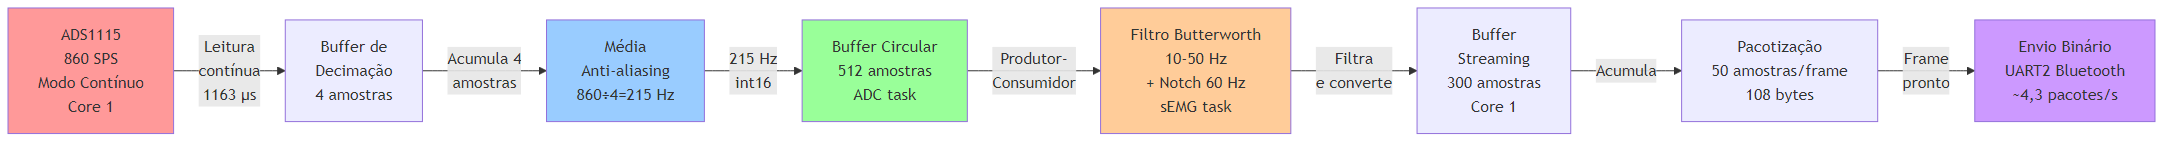
\includegraphics[width=\textwidth]{figuras/Desenvolvimento/NeuroEstimulator/pipeline-aquisicao-decimacao.png}
    \fonte{Autoria própria (2026)}
\end{figure}

% ----------------------------------------------------------------------
\subsubsection{Reorganização das tarefas FreeRTOS}\label{subsubsec:NETarefas}
% ----------------------------------------------------------------------

A operação contínua do estágio de aquisição inviabilizou o modelo original do \textit{firmware}, no qual uma única função de \textit{callback} disparada por temporizador realizava a leitura síncrona do ADC, aplicava o filtro e empacotava o dado para envio via Bluetooth. Esse modelo monolítico bloqueava o núcleo durante o intervalo de leitura I$^2$C do ADS1115 e, sob carga (por exemplo, durante a transmissão de respostas JSON pela mesma UART), provocava perda sistemática de amostras. A solução foi decompor o caminho do dado em uma cadeia produtor-consumidor de três tarefas FreeRTOS distintas, distribuídas entre os dois núcleos do ESP32 e desacopladas por buffers circulares.

No núcleo destinado às operações sensíveis a temporização do estímulo (\textit{Core 0}), permaneceram a tarefa de gestão da sessão de FES (prioridade 20) e a tarefa sensora legada empregada na detecção de gatilho mioelétrico para disparo do estímulo (prioridade 10). No núcleo dedicado à comunicação (\textit{Core 1}) passaram a coexistir três tarefas: a tarefa de tratamento de mensagens Bluetooth (prioridade 20), a tarefa de aquisição contínua do ADC (prioridade 18) e a tarefa de \textit{streaming} de sEMG (prioridade 15). A distribuição de prioridades reflete a hierarquia funcional desejada: o tratamento de comandos do aplicativo precede o consumo de dados do conversor, que por sua vez precede a entrega ao canal de saída. As três tarefas do núcleo de comunicação compartilham os recursos de \textit{hardware} por meio de dois \textit{mutexes}: o \texttt{i2cMutex}, que serializa o acesso ao barramento I$^2$C (compartilhado com o giroscópio MPU6050), e o \texttt{MutexBlu}, que serializa a escrita na UART2 entre a tarefa de \textit{streaming} e o tratador de mensagens, evitando entrelaçamento de \textit{bytes} no canal Bluetooth.

O acoplamento entre as tarefas de aquisição e de \textit{streaming} é feito por um buffer circular de 512 amostras de 16 \textit{bits}, dimensionado para tolerar rajadas de mais de dois segundos sem perda; já o acoplamento entre a etapa de filtragem digital e a pacotização para Bluetooth utiliza um segundo buffer circular de 300 amostras, suficiente para absorver atrasos de transmissão de até aproximadamente 1,4\,segundo. Em ambos os buffers, a estratégia de tratamento de \textit{overflow} é o descarte da amostra mais antiga (\textit{drop-oldest}) com sinalização por \textit{log} limitada a uma ocorrência por segundo, escolha que privilegia a continuidade do fluxo em detrimento da bloqueio do produtor -- um dispositivo de aquisição de sEMG que pausa para esperar o consumidor é, na prática, indistinguível de um dispositivo defeituoso para o operador no aplicativo.

A Figura~\ref{fig:tasksFreertos} apresenta a topologia resultante e destaca as relações produtor-consumidor entre as tarefas. Como melhoria adicional, o procedimento de encerramento das tarefas (\textit{shutdown} cooperativo) foi reescrito para sinalizar uma \textit{flag} volátil de saída e aguardar o término natural da iteração corrente antes de remover a tarefa, em substituição ao \texttt{vTaskDelete} direto que o \textit{firmware} original utilizava. A motivação foi eliminar uma classe específica de defeitos observada em sessões consecutivas de aquisição, na qual a remoção da tarefa em meio a uma transação I$^2$C corrompia o estado interno do barramento e exigia reinicialização física do dispositivo.

\begin{figure}[htb]
    \caption{Topologia das tarefas FreeRTOS no \textit{firmware} adaptado}
    \label{fig:tasksFreertos}
    \centering
    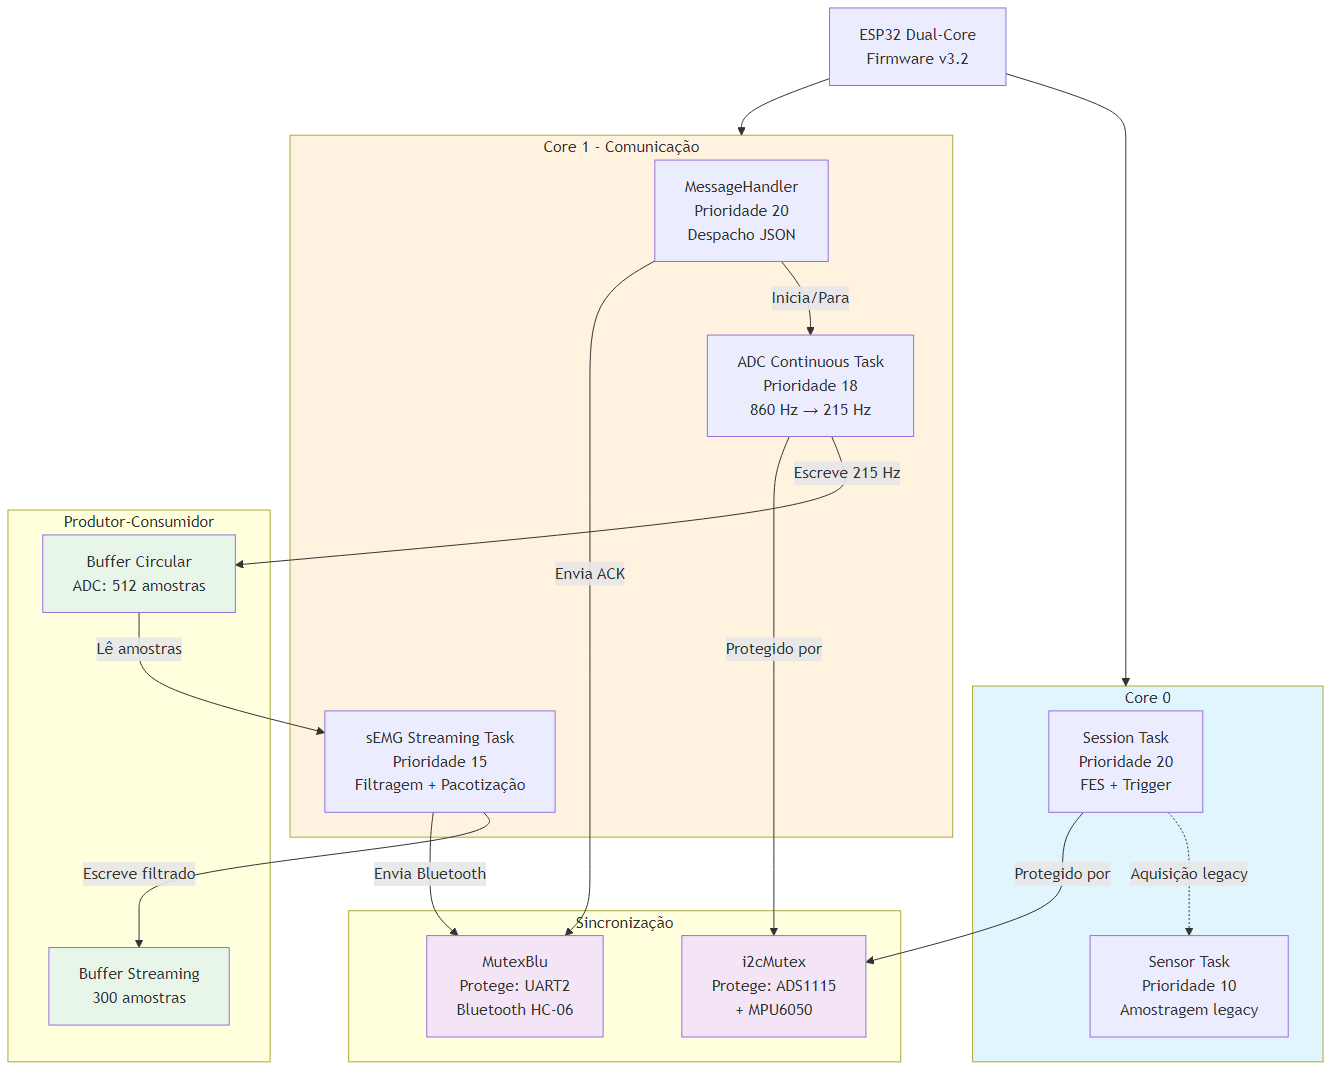
\includegraphics[width=\textwidth]{figuras/Desenvolvimento/NeuroEstimulator/tasks-freertos.png}
    \fonte{Autoria própria (2026)}
\end{figure}

% ----------------------------------------------------------------------
\subsubsection{Protocolo Bluetooth: do comando-resposta ao \textit{streaming}}\label{subsubsec:NEProtocolo}
% ----------------------------------------------------------------------

O protocolo de comunicação do \textit{firmware} original era inteiramente baseado em mensagens JSON encapsuladas em um envelope \verb|{"cd": <code>, "mt": "<method>", "bd": {...}}| trafegando sobre a UART2. Para a aquisição de sEMG, o aplicativo enviava periodicamente uma requisição de leitura e o \textit{firmware} respondia com um pequeno bloco de amostras codificado em JSON. Esse padrão tem dois inconvenientes em uma aplicação de \textit{streaming}: o aplicativo precisa manter um relógio sincronizado com o \textit{firmware} apenas para temporizar suas requisições, e a redundância textual do JSON (chaves de objeto, vírgulas, representação decimal de cada amostra como \textit{string}) consome largura de banda desproporcional à informação efetivamente transportada.

No \textit{firmware} adaptado, o protocolo passou a ser dual: comandos de controle continuam em JSON, mantendo legibilidade e compatibilidade com ferramentas existentes; o fluxo de dados de sEMG, entretanto, é transmitido como uma sequência de pacotes binários enviados de forma autônoma pelo \textit{firmware} entre as transições \texttt{START\_STREAM} e \texttt{STOP\_STREAM}. O aplicativo abre o \textit{streaming} enviando \verb|{"cd":11,"mt":"x"}|, recebe um \textit{acknowledgment} \verb|{"cd":11,"mt":"a"}| e, a partir desse momento, recebe pacotes binários até enviar \verb|{"cd":12,"mt":"x"}| para encerrar. A transição inversa -- voltar a um modelo comando-resposta para o canal de dados -- foi descartada como design alternativo, em razão das desvantagens já discutidas; a configuração de taxa em tempo de execução, presente em uma versão intermediária do \textit{firmware} sob o código de mensagem \texttt{cd:14}, também foi removida, em favor da configuração fixa de 215\,SPS discutida na Subseção~\ref{subsubsec:NEDecimacao}. O Quadro~\ref{quad:campos-pacote-binario} descreve os campos do novo \textit{frame} de dados, e a Figura~\ref{fig:pacoteBinario} ilustra graficamente seu \textit{layout}.

\begin{table}[htb]
    \centering
    \caption{Quadro -- Campos do pacote binário de \textit{streaming} de sEMG}\label{tab:campos-pacote-binario}
    \begin{tabular}{|c|c|l|p{6cm}|}
        \hline
        \textbf{Offset} & \textbf{Tamanho} & \textbf{Campo} & \textbf{Descrição} \\
        \hline
        0 & 1 \textit{byte} & \texttt{magic} & Marcador de início de pacote (valor fixo \texttt{0xAA}). \\
        \hline
        1 & 1 \textit{byte} & \texttt{message\_code} & Código do tipo de mensagem (valor fixo \texttt{0x0D}, dados de \textit{stream}). \\
        \hline
        2 & 4 \textit{bytes} & \texttt{timestamp} & Valor de \texttt{millis()} no ESP32, em \textit{little-endian}. \\
        \hline
        6 & 2 \textit{bytes} & \texttt{sample\_count} & Número de amostras no \textit{payload} (tipicamente 50). \\
        \hline
        8 & 100 \textit{bytes} & \texttt{samples[]} & 50 valores \texttt{int16\_t} em \textit{little-endian} (1\,LSB $\equiv$ 1\,mV). \\
        \hline
        \multicolumn{2}{|c|}{\textbf{Total: 108 \textit{bytes}}} & \multicolumn{2}{l|}{\textit{Frame} fixo enviado a $\approx$\,4,3 pacotes/s.} \\
        \hline
    \end{tabular}
    \fonte{Autoria própria (2026)}
\end{table}

\begin{figure}[htb]
    \caption{\textit{Layout} binário do pacote de \textit{streaming}}
    \label{fig:pacoteBinario}
    \centering
    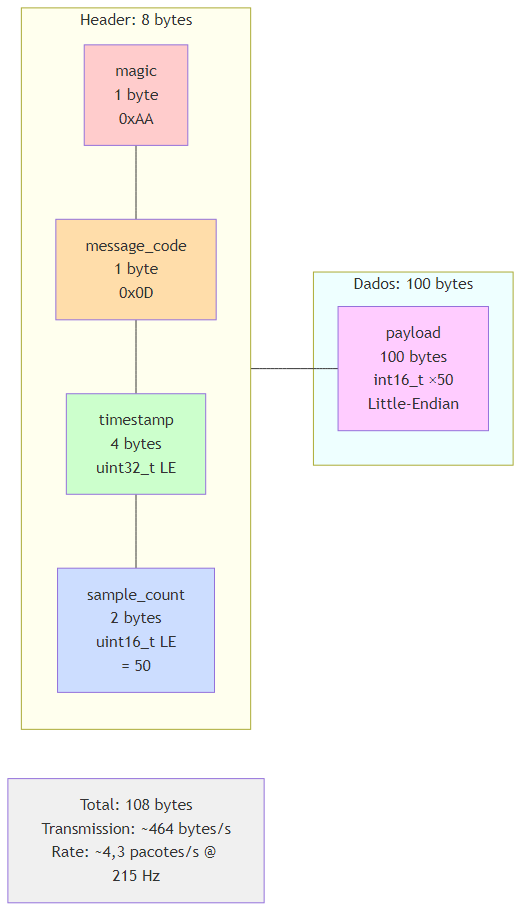
\includegraphics[width=0.95\textwidth]{figuras/Desenvolvimento/NeuroEstimulator/pacote-binario.png}
    \fonte{Autoria própria (2026)}
\end{figure}

A Figura~\ref{fig:protocoloStreaming} resume o diálogo completo entre o IRIS Mobile, o tratador de mensagens, as tarefas internas do \textit{firmware} e o canal Bluetooth durante uma sessão de aquisição.

\begin{figure}[htb]
    \caption{Diagrama de sequência do \textit{streaming} de sEMG entre o IRIS Mobile e o \textit{firmware} adaptado}
    \label{fig:protocoloStreaming}
    \centering
    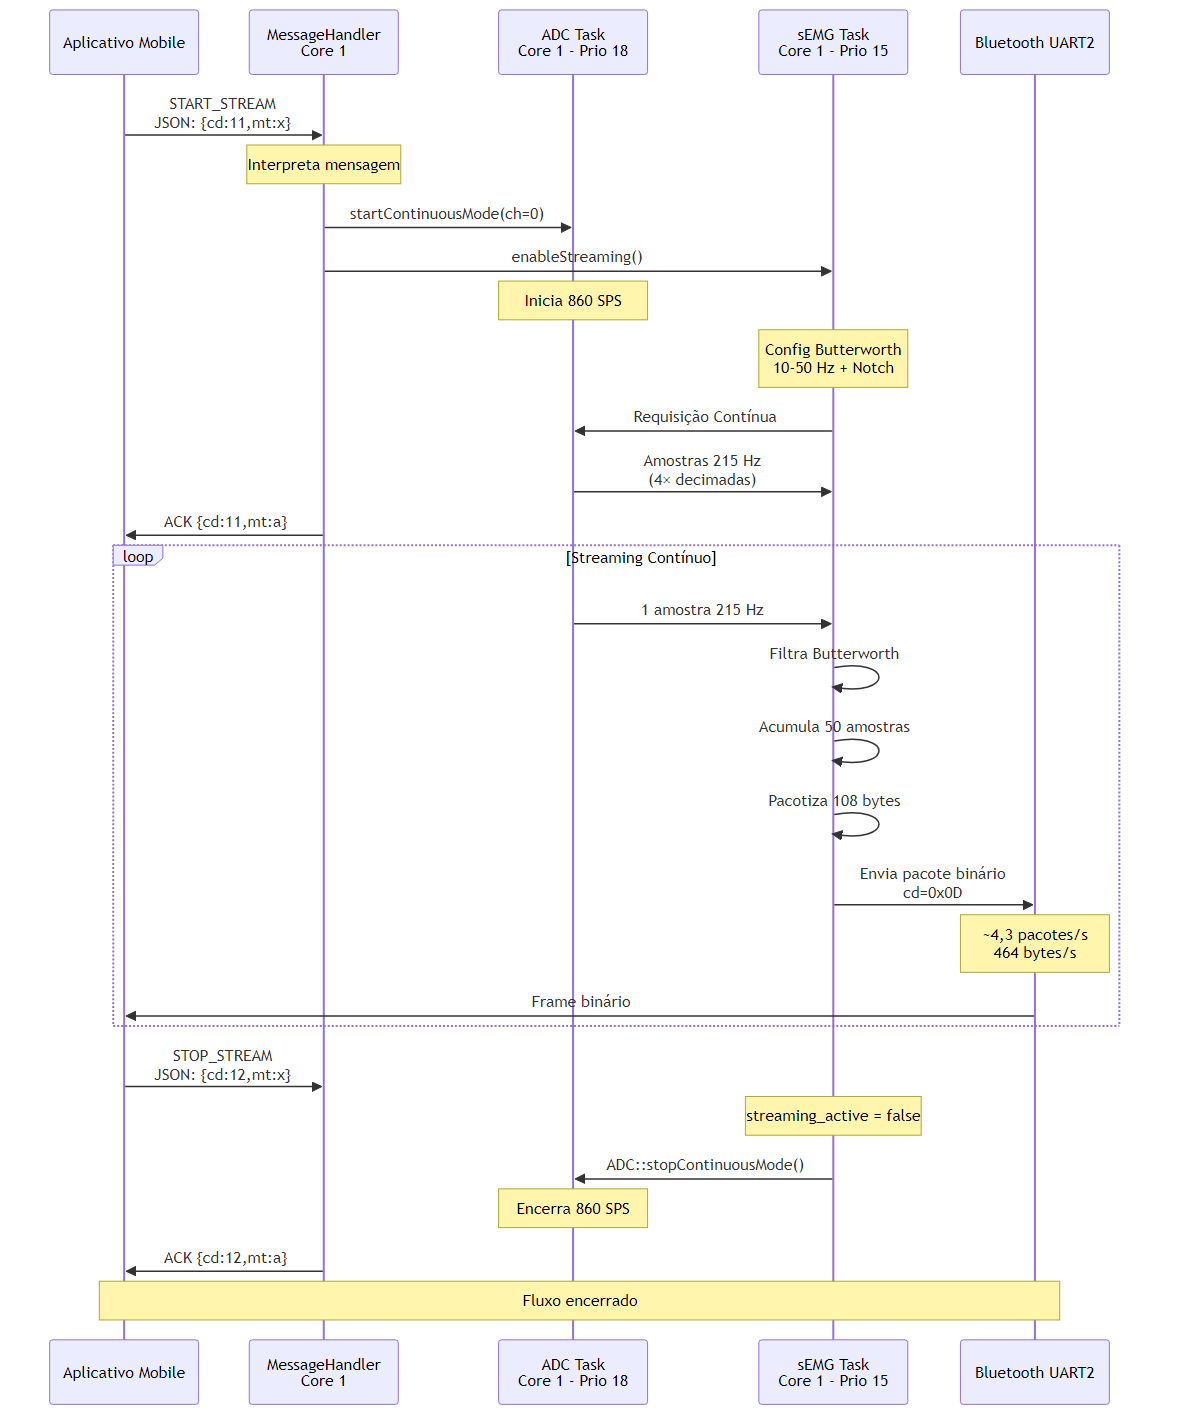
\includegraphics[width=\textwidth]{figuras/Desenvolvimento/NeuroEstimulator/protocolo-streaming.png}
    \fonte{Autoria própria (2026)}
\end{figure}

A escolha de codificar cada amostra em \texttt{int16\_t}, em vez de ponto flutuante, e de \textit{little-endian} como ordem de \textit{bytes} foi guiada por três critérios: a preservação da precisão útil do sinal (a granularidade do ADS1115 a 16~\textit{bits} permite representar tensões em milivolts inteiros sem perda significativa para a aplicação); a economia de banda em relação às alternativas textuais (a transmissão equivalente em JSON consumiria mais do que o triplo da capacidade do canal a 215\,SPS); e a interoperabilidade com a arquitetura nativa do ESP32 e dos dispositivos móveis modernos, que são predominantemente \textit{little-endian} -- o que evita conversões de ordem de \textit{byte} no consumidor. A compatibilidade retroativa com o protocolo JSON anterior para o canal de dados foi descartada de forma deliberada: aplicações que ainda dependam do formato textual podem consumir o canal de controle, mas o IRIS Mobile e o NPI consomem exclusivamente o protocolo binário aqui descrito.

% ======================================================================
% Lista de placeholders de imagens sugeridas (referência interna -- não
% renderizada). Cada item indica o caminho esperado e o que a imagem
% deve mostrar:
% ----------------------------------------------------------------------
% [1] figuras/Desenvolvimento/NeuroEstimulator/neuroestimulador-foto.jpg
%     Foto frontal do dispositivo NeuroEstimulator (caixa MDF, botão de
%     emergência, LEDs de status, conectores). Sugestão: reaproveitar a
%     Figura 7 do Technical Report -- Integration Workshop 3 (2023) ou
%     produzir uma fotografia atualizada. Referenciada (em comentário) em
%     \subsec{NEOriginal}.
%
% [2] figuras/Desenvolvimento/NeuroEstimulator/pipeline-aquisicao-decimacao.png
%     Renderização PNG do diagrama Mermaid pipeline-aquisicao-decimacao.mmd
%     (já existente). Mostra ADS1115 -> média 4x -> buffer circular ->
%     filtros -> buffer streaming -> pacote binário -> Bluetooth.
%
% [3] figuras/Desenvolvimento/NeuroEstimulator/tasks-freertos.png
%     Renderização PNG do diagrama Mermaid tasks-freertos.mmd
%     (já existente). Mostra topologia FreeRTOS pos-refatoracao,
%     com Core 0 / Core 1, prioridades e mutexes.
%
% [4] figuras/Desenvolvimento/NeuroEstimulator/protocolo-streaming.png
%     Renderização PNG do diagrama Mermaid protocolo-streaming.mmd
%     (já existente). Mostra sequencia START_STREAM -> ACK -> pacotes
%     binarios autonomos -> STOP_STREAM -> ACK.
%
% [5] figuras/Desenvolvimento/NeuroEstimulator/pacote-binario.png
%     Renderização PNG do diagrama Mermaid pacote-binario.mmd
%     (já existente). Mostra layout do frame de 108 bytes com header
%     (magic, code, timestamp, sample_count) e payload (50 x int16_t).
% ======================================================================

% =====================================================================

\section{Adaptação do NeuroEstimulator}\label{sec:adaptacaoNeuroEstimulator}

O NeuroEstimulator descrito na Seção~\ref{sec:coletaDeDados} foi adotado, no presente trabalho, como dispositivo-exemplo para validar a integração de equipamentos de aquisição de biossinais ao PRISM. A descrição original do projeto -- mecânica, eletrônica, escolha de componentes e arquitetura geral do firmware -- não é repetida aqui; esta seção concentra-se exclusivamente nas \textbf{modificações} introduzidas para tornar o dispositivo compatível com o fluxo de etiquetagem em tempo real previsto pelo IRIS Mobile e, consequentemente, com o modelo de coleta padronizado proposto pelo PRISM. As alterações foram restritas ao firmware e ao protocolo de comunicação Bluetooth: nenhuma modificação foi feita na placa de circuito impresso, no \textit{front-end} analógico, no transformador 1:10 ou nos elementos mecânicos do equipamento.

% ----------------------------------------------------------------------
\subsection{O dispositivo original}\label{subsec:NEOriginal}
% ----------------------------------------------------------------------

Para fins de contextualização, recapitulam-se aqui apenas os elementos do dispositivo original relevantes para a adaptação. O NeuroEstimulator é um sistema funcional de eletroestimulação descrito em detalhes na Seção~\ref{sec:coletaDeDados}, organizado em torno de um microcontrolador ESP32 (arquitetura Xtensa LX6 \textit{dual-core}), \textit{front-end} analógico AD8232 dedicado à condicionamento do sinal de eletromiografia de superfície (sEMG), conversor analógico-digital ADS1115 (16 bits de resolução, taxa máxima de 860 amostras por segundo na configuração utilizada) e módulo Bluetooth Classic HC-06 acoplado à UART2. O \textit{firmware} originalmente embarcado opera sobre o sistema operacional de tempo real FreeRTOS, distribuindo entre os dois núcleos do ESP32 as tarefas de gestão de sessão, geração de pulsos de estimulação elétrica funcional (FES, do inglês \textit{Functional Electrical Stimulation}) e leitura periódica do sEMG.

% Imagem sugerida: foto do dispositivo montado (caixa MDF + PCB + suportes).
% Este placeholder permite reutilizar a Figura~7 do relatório técnico do
% Workshop de Integração 3 (NeuroEstimulator, 2023) ou capturar uma nova
% fotografia atualizada do equipamento.
%
% \begin{figure}[htb]
%     \caption{Visão externa do NeuroEstimulator utilizado como dispositivo-exemplo}
%     \label{fig:neuroEstimuladorExterno}
%     \centering
%     \includegraphics[width=0.7\textwidth]{figuras/Desenvolvimento/NeuroEstimulator/neuroestimulador-foto.jpg}
%     \fonte{}
% \end{figure}

% ----------------------------------------------------------------------
\subsection{Diferencial pretendido para o trabalho}\label{subsec:NERequisitos}
% ----------------------------------------------------------------------

A adoção do NeuroEstimulator como dispositivo-exemplo do PRISM exigiu uma reformulação parcial do \textit{firmware} para satisfazer requisitos que não eram contemplados pelo projeto original. Esses requisitos derivam diretamente do modelo de coleta proposto, em que o sinal de sEMG precisa ser exibido e etiquetado em tempo real pelo IRIS Mobile durante a sessão. As principais diretrizes que motivaram a refatoração foram:

\begin{enumerate}
    \item \textbf{Maximizar a taxa efetiva de amostragem entregue ao aplicativo}, aproximando-a do limite teórico do conversor empregado e estabilizando-a em um valor previsível. Na implementação anterior do \textit{firmware}, o pareamento entre o temporizador de amostragem e a leitura síncrona do ADS1115 causava bloqueios da ordem de milissegundos, fazendo com que apenas uma fração das amostras nominalmente programadas chegasse efetivamente ao aplicativo;
    \item \textbf{Substituir o protocolo do tipo comando-resposta} por uma transmissão contínua orientada a fluxo (\textit{streaming}), de modo que cada amostra coletada seja entregue ao consumidor sem necessidade de requisição explícita;
    \item \textbf{Tornar o contrato de comunicação compatível com a etiquetagem em tempo real} prevista pelo IRIS Mobile, agregando carimbo de tempo (\textit{timestamp}) consistente em cada bloco de amostras e reduzindo a sobrecarga de transporte para que o canal serial Bluetooth não se tornasse o gargalo do sistema;
    \item \textbf{Manter a compatibilidade com o \textit{hardware} existente}, sem qualquer alteração na placa, no \textit{front-end} analógico, no estágio de potência da estimulação ou no módulo Bluetooth Classic já instalado.
\end{enumerate}

Os três primeiros requisitos pertencem ao domínio do \textit{software} embarcado e do protocolo. O quarto é uma restrição de projeto que limita o universo de soluções possíveis -- em particular, ele inviabiliza a substituição do ADS1115 por um conversor de taxa mais alta e impede a troca do HC-06 por um módulo Bluetooth Low Energy ou Wi-Fi de maior largura de banda.

% ----------------------------------------------------------------------
\subsection{Modificações no firmware}\label{subsec:NEFirmware}
% ----------------------------------------------------------------------

As modificações no \textit{firmware} foram organizadas em três frentes complementares, descritas nas próximas subseções: a reconfiguração do estágio de aquisição para operar em modo contínuo com decimação interna; a reorganização das tarefas FreeRTOS em um pipeline produtor-consumidor; e a substituição do protocolo Bluetooth comando-resposta por um \textit{streaming} binário com cabeçalho fixo.

% ----------------------------------------------------------------------
\subsubsection{Aquisição contínua a 860 SPS e decimação para 215 SPS}\label{subsubsec:NEDecimacao}
% ----------------------------------------------------------------------

A taxa efetiva de saída do estágio de aquisição foi fixada em 215 amostras por segundo (\textit{samples per second}, SPS), obtida a partir de uma operação contínua do ADS1115 a 860 SPS seguida de uma decimação 4:1 por média móvel. A escolha de 860 SPS como ponto de operação não é arbitrária: trata-se da maior taxa nominal disponível no ADS1115 quando configurado em modo de conversão contínua com a faixa de tensão de entrada utilizada pelo NeuroEstimulator. Operar abaixo desse teto deixaria capacidade ociosa do conversor; tentar ultrapassá-lo simplesmente não é suportado pelo \textit{hardware}.

A decimação 4:1 por média foi adotada por três razões. A primeira é o seu efeito como filtro \textit{anti-aliasing} simples: o cálculo da média de quatro amostras consecutivas atenua componentes de alta frequência antes que o sinal seja entregue à etapa de filtragem digital, reduzindo a probabilidade de \textit{aliasing} causado por ruído eletromagnético do ambiente clínico. A segunda razão é a obtenção de uma relação 1:1 entre amostras lidas e amostras entregues que respeita os limites de banda exigidos pelo canal Bluetooth Classic: a 215 SPS, com codificação binária compacta, a vazão de saída fica em torno de 464 \textit{bytes} por segundo, o que corresponde a aproximadamente 4\% da capacidade nominal da UART2 configurada a 115\,200 \textit{baud}, deixando uma margem confortável para retransmissões e tráfego de controle. A terceira razão é simplificar a configuração do filtro digital: ao fixar a taxa de entrega em 215 SPS, os coeficientes do filtro Butterworth de segunda ordem (passa-faixa de 10\,Hz a 50\,Hz) e do \textit{notch} de 60\,Hz para rejeição de interferência da rede elétrica podem ser pré-calculados em tempo de compilação, eliminando uma fonte recorrente de erros que o \textit{firmware} original apresentava ao reconfigurar dinamicamente a taxa.

É necessário, contudo, discutir honestamente a contrapartida dessa escolha. A literatura de eletromiografia indica que a banda útil do sEMG de superfície estende-se aproximadamente entre 10\,Hz e 500\,Hz. Pelo critério de Nyquist, uma taxa de amostragem efetiva de 215 SPS limita a banda passível de reconstrução fiel a aproximadamente 107,5\,Hz, valor inferior ao extremo superior da banda fisiológica do sEMG. A decisão arquitetural foi privilegiar a faixa entre 10\,Hz e 50\,Hz, onde se concentra a maior parte da energia do sinal mioelétrico utilizado para detecção de ativação muscular, em detrimento da captura de componentes de mais alta frequência. Esta limitação é uma decorrência direta da restrição de não modificar o \textit{hardware} (Subseção~\ref{subsec:NERequisitos}, requisito 4); ela é retomada no capítulo de discussão dos resultados à luz dos sinais efetivamente capturados, e deve ser entendida como uma limitação reconhecida do dispositivo-exemplo, não uma propriedade do PRISM.

A Figura~\ref{fig:pipelineAquisicaoDecimacao} resume o caminho do dado desde o conversor analógico-digital até a saída pelo módulo Bluetooth.

\begin{figure}[htb]
    \caption{Pipeline de aquisição, decimação e filtragem do sEMG no \textit{firmware} adaptado}
    \label{fig:pipelineAquisicaoDecimacao}
    \centering
    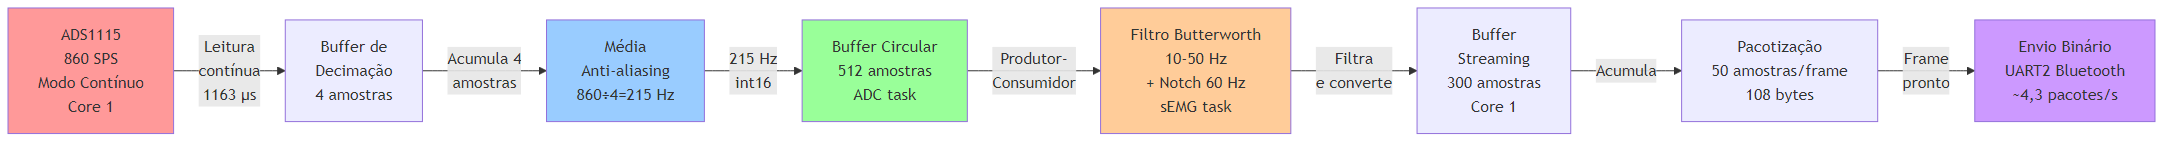
\includegraphics[width=\textwidth]{figuras/Desenvolvimento/NeuroEstimulator/pipeline-aquisicao-decimacao.png}
    \fonte{Autoria própria (2026)}
\end{figure}

% ----------------------------------------------------------------------
\subsubsection{Reorganização das tarefas FreeRTOS}\label{subsubsec:NETarefas}
% ----------------------------------------------------------------------

A operação contínua do estágio de aquisição inviabilizou o modelo original do \textit{firmware}, no qual uma única função de \textit{callback} disparada por temporizador realizava a leitura síncrona do ADC, aplicava o filtro e empacotava o dado para envio via Bluetooth. Esse modelo monolítico bloqueava o núcleo durante o intervalo de leitura I$^2$C do ADS1115 e, sob carga (por exemplo, durante a transmissão de respostas JSON pela mesma UART), provocava perda sistemática de amostras. A solução foi decompor o caminho do dado em uma cadeia produtor-consumidor de três tarefas FreeRTOS distintas, distribuídas entre os dois núcleos do ESP32 e desacopladas por buffers circulares.

No núcleo destinado às operações sensíveis a temporização do estímulo (\textit{Core 0}), permaneceram a tarefa de gestão da sessão de FES (prioridade 20) e a tarefa sensora legada empregada na detecção de gatilho mioelétrico para disparo do estímulo (prioridade 10). No núcleo dedicado à comunicação (\textit{Core 1}) passaram a coexistir três tarefas: a tarefa de tratamento de mensagens Bluetooth (prioridade 20), a tarefa de aquisição contínua do ADC (prioridade 18) e a tarefa de \textit{streaming} de sEMG (prioridade 15). A distribuição de prioridades reflete a hierarquia funcional desejada: o tratamento de comandos do aplicativo precede o consumo de dados do conversor, que por sua vez precede a entrega ao canal de saída. As três tarefas do núcleo de comunicação compartilham os recursos de \textit{hardware} por meio de dois \textit{mutexes}: o \texttt{i2cMutex}, que serializa o acesso ao barramento I$^2$C (compartilhado com o giroscópio MPU6050), e o \texttt{MutexBlu}, que serializa a escrita na UART2 entre a tarefa de \textit{streaming} e o tratador de mensagens, evitando entrelaçamento de \textit{bytes} no canal Bluetooth.

O acoplamento entre as tarefas de aquisição e de \textit{streaming} é feito por um buffer circular de 512 amostras de 16 \textit{bits}, dimensionado para tolerar rajadas de mais de dois segundos sem perda; já o acoplamento entre a etapa de filtragem digital e a pacotização para Bluetooth utiliza um segundo buffer circular de 300 amostras, suficiente para absorver atrasos de transmissão de até aproximadamente 1,4\,segundo. Em ambos os buffers, a estratégia de tratamento de \textit{overflow} é o descarte da amostra mais antiga (\textit{drop-oldest}) com sinalização por \textit{log} limitada a uma ocorrência por segundo, escolha que privilegia a continuidade do fluxo em detrimento da bloqueio do produtor -- um dispositivo de aquisição de sEMG que pausa para esperar o consumidor é, na prática, indistinguível de um dispositivo defeituoso para o operador no aplicativo.

A Figura~\ref{fig:tasksFreertos} apresenta a topologia resultante e destaca as relações produtor-consumidor entre as tarefas. Como melhoria adicional, o procedimento de encerramento das tarefas (\textit{shutdown} cooperativo) foi reescrito para sinalizar uma \textit{flag} volátil de saída e aguardar o término natural da iteração corrente antes de remover a tarefa, em substituição ao \texttt{vTaskDelete} direto que o \textit{firmware} original utilizava. A motivação foi eliminar uma classe específica de defeitos observada em sessões consecutivas de aquisição, na qual a remoção da tarefa em meio a uma transação I$^2$C corrompia o estado interno do barramento e exigia reinicialização física do dispositivo.

\begin{figure}[htb]
    \caption{Topologia das tarefas FreeRTOS no \textit{firmware} adaptado}
    \label{fig:tasksFreertos}
    \centering
    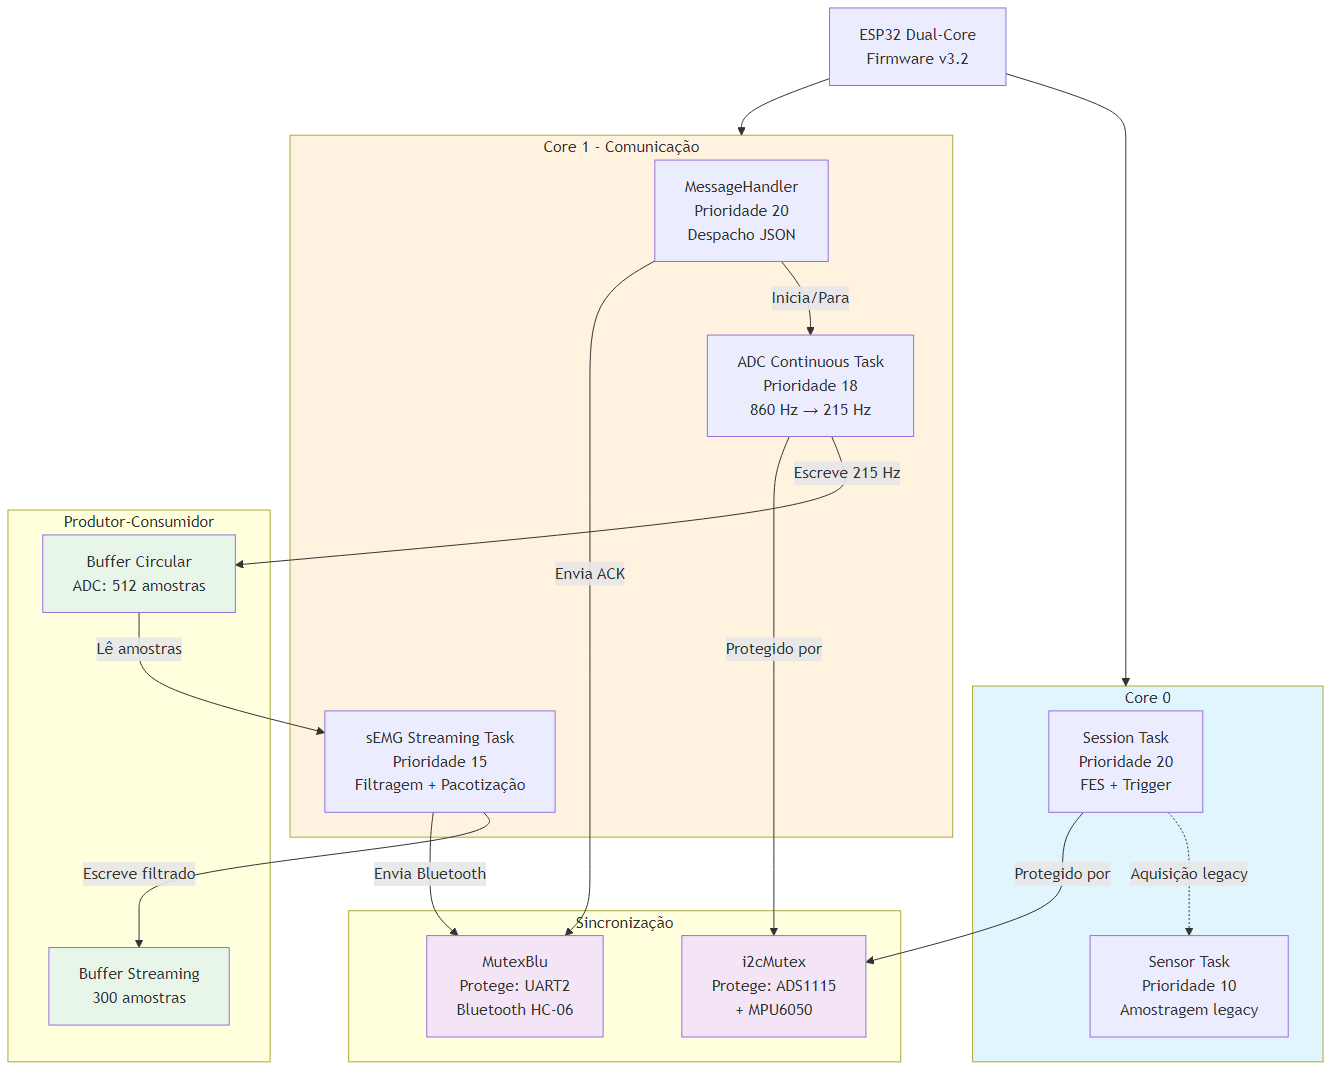
\includegraphics[width=\textwidth]{figuras/Desenvolvimento/NeuroEstimulator/tasks-freertos.png}
    \fonte{Autoria própria (2026)}
\end{figure}

% ----------------------------------------------------------------------
\subsubsection{Protocolo Bluetooth: do comando-resposta ao \textit{streaming}}\label{subsubsec:NEProtocolo}
% ----------------------------------------------------------------------

O protocolo de comunicação do \textit{firmware} original era inteiramente baseado em mensagens JSON encapsuladas em um envelope \verb|{"cd": <code>, "mt": "<method>", "bd": {...}}| trafegando sobre a UART2. Para a aquisição de sEMG, o aplicativo enviava periodicamente uma requisição de leitura e o \textit{firmware} respondia com um pequeno bloco de amostras codificado em JSON. Esse padrão tem dois inconvenientes em uma aplicação de \textit{streaming}: o aplicativo precisa manter um relógio sincronizado com o \textit{firmware} apenas para temporizar suas requisições, e a redundância textual do JSON (chaves de objeto, vírgulas, representação decimal de cada amostra como \textit{string}) consome largura de banda desproporcional à informação efetivamente transportada.

No \textit{firmware} adaptado, o protocolo passou a ser dual: comandos de controle continuam em JSON, mantendo legibilidade e compatibilidade com ferramentas existentes; o fluxo de dados de sEMG, entretanto, é transmitido como uma sequência de pacotes binários enviados de forma autônoma pelo \textit{firmware} entre as transições \texttt{START\_STREAM} e \texttt{STOP\_STREAM}. O aplicativo abre o \textit{streaming} enviando \verb|{"cd":11,"mt":"x"}|, recebe um \textit{acknowledgment} \verb|{"cd":11,"mt":"a"}| e, a partir desse momento, recebe pacotes binários até enviar \verb|{"cd":12,"mt":"x"}| para encerrar. A transição inversa -- voltar a um modelo comando-resposta para o canal de dados -- foi descartada como design alternativo, em razão das desvantagens já discutidas; a configuração de taxa em tempo de execução, presente em uma versão intermediária do \textit{firmware} sob o código de mensagem \texttt{cd:14}, também foi removida, em favor da configuração fixa de 215\,SPS discutida na Subseção~\ref{subsubsec:NEDecimacao}. O Quadro~\ref{quad:campos-pacote-binario} descreve os campos do novo \textit{frame} de dados, e a Figura~\ref{fig:pacoteBinario} ilustra graficamente seu \textit{layout}.

\begin{table}[htb]
    \centering
    \caption{Quadro -- Campos do pacote binário de \textit{streaming} de sEMG}\label{tab:campos-pacote-binario}
    \begin{tabular}{|c|c|l|p{6cm}|}
        \hline
        \textbf{Offset} & \textbf{Tamanho} & \textbf{Campo} & \textbf{Descrição} \\
        \hline
        0 & 1 \textit{byte} & \texttt{magic} & Marcador de início de pacote (valor fixo \texttt{0xAA}). \\
        \hline
        1 & 1 \textit{byte} & \texttt{message\_code} & Código do tipo de mensagem (valor fixo \texttt{0x0D}, dados de \textit{stream}). \\
        \hline
        2 & 4 \textit{bytes} & \texttt{timestamp} & Valor de \texttt{millis()} no ESP32, em \textit{little-endian}. \\
        \hline
        6 & 2 \textit{bytes} & \texttt{sample\_count} & Número de amostras no \textit{payload} (tipicamente 50). \\
        \hline
        8 & 100 \textit{bytes} & \texttt{samples[]} & 50 valores \texttt{int16\_t} em \textit{little-endian} (1\,LSB $\equiv$ 1\,mV). \\
        \hline
        \multicolumn{2}{|c|}{\textbf{Total: 108 \textit{bytes}}} & \multicolumn{2}{l|}{\textit{Frame} fixo enviado a $\approx$\,4,3 pacotes/s.} \\
        \hline
    \end{tabular}
    \fonte{Autoria própria (2026)}
\end{table}

\begin{figure}[htb]
    \caption{\textit{Layout} binário do pacote de \textit{streaming}}
    \label{fig:pacoteBinario}
    \centering
    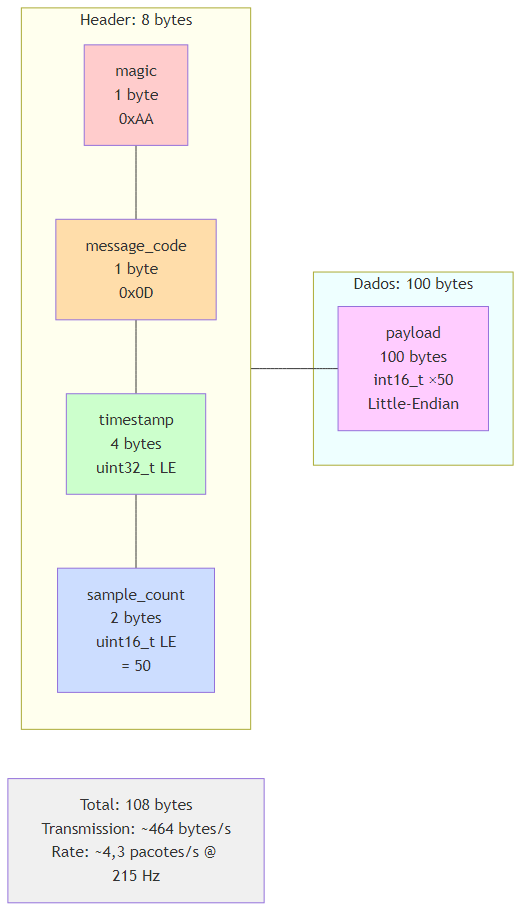
\includegraphics[width=0.95\textwidth]{figuras/Desenvolvimento/NeuroEstimulator/pacote-binario.png}
    \fonte{Autoria própria (2026)}
\end{figure}

A Figura~\ref{fig:protocoloStreaming} resume o diálogo completo entre o IRIS Mobile, o tratador de mensagens, as tarefas internas do \textit{firmware} e o canal Bluetooth durante uma sessão de aquisição.

\begin{figure}[htb]
    \caption{Diagrama de sequência do \textit{streaming} de sEMG entre o IRIS Mobile e o \textit{firmware} adaptado}
    \label{fig:protocoloStreaming}
    \centering
    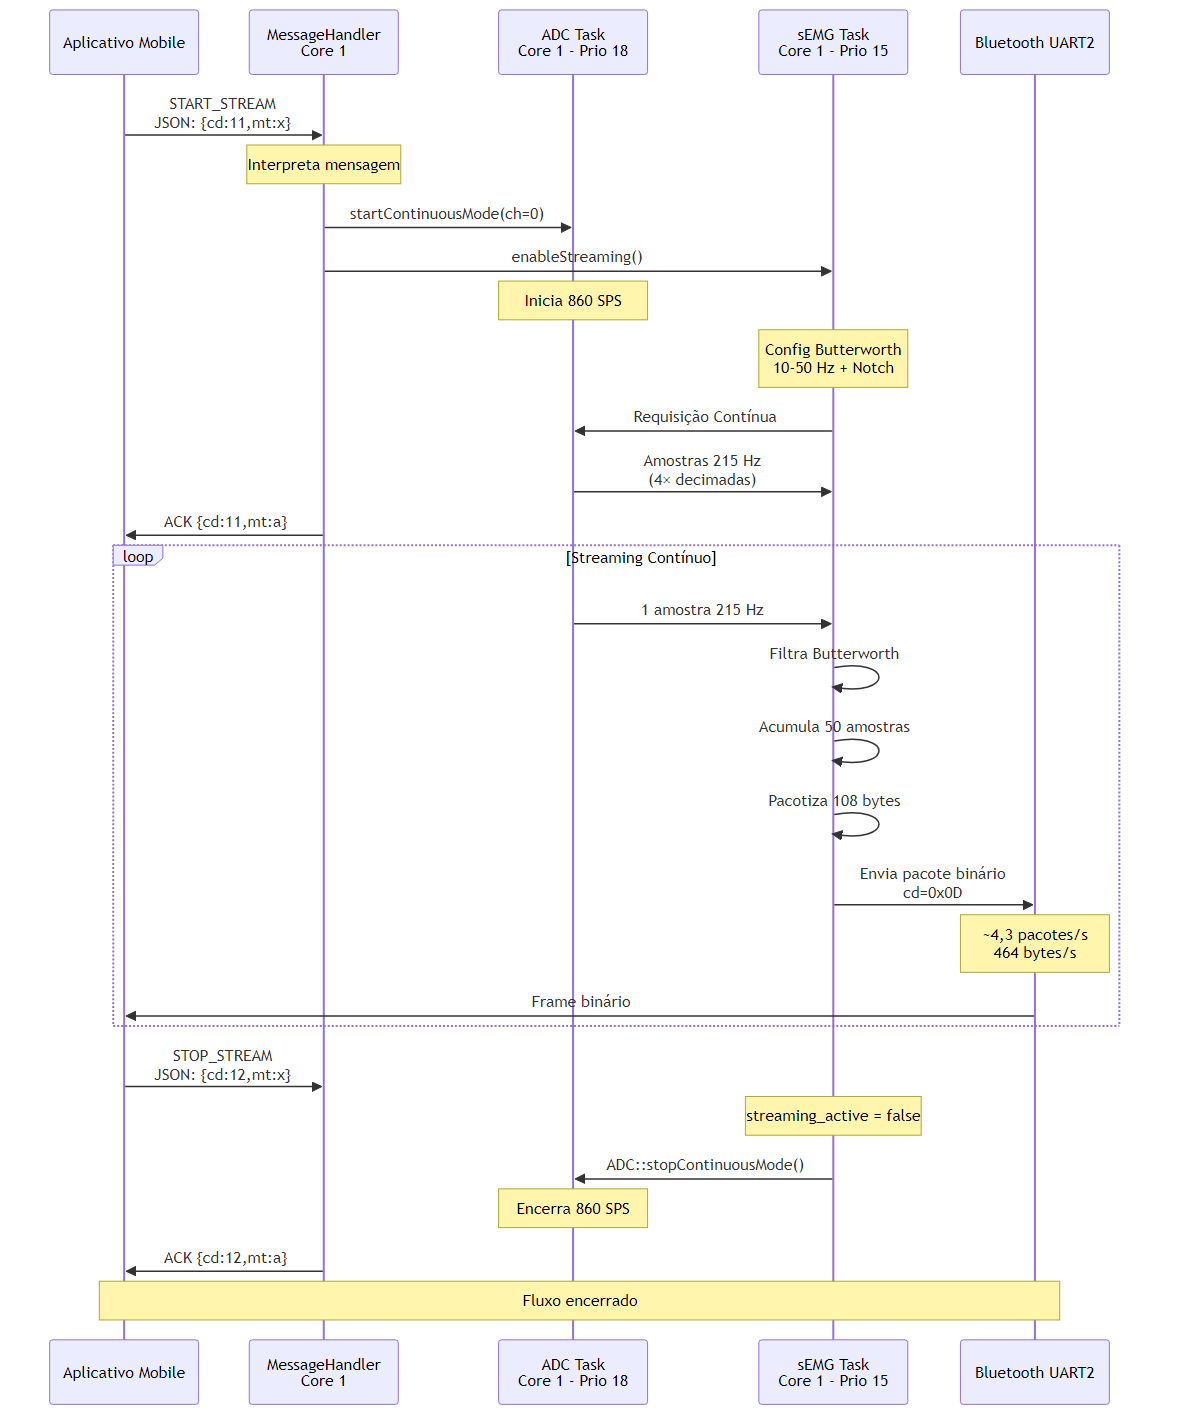
\includegraphics[width=\textwidth]{figuras/Desenvolvimento/NeuroEstimulator/protocolo-streaming.png}
    \fonte{Autoria própria (2026)}
\end{figure}

A escolha de codificar cada amostra em \texttt{int16\_t}, em vez de ponto flutuante, e de \textit{little-endian} como ordem de \textit{bytes} foi guiada por três critérios: a preservação da precisão útil do sinal (a granularidade do ADS1115 a 16~\textit{bits} permite representar tensões em milivolts inteiros sem perda significativa para a aplicação); a economia de banda em relação às alternativas textuais (a transmissão equivalente em JSON consumiria mais do que o triplo da capacidade do canal a 215\,SPS); e a interoperabilidade com a arquitetura nativa do ESP32 e dos dispositivos móveis modernos, que são predominantemente \textit{little-endian} -- o que evita conversões de ordem de \textit{byte} no consumidor. A compatibilidade retroativa com o protocolo JSON anterior para o canal de dados foi descartada de forma deliberada: aplicações que ainda dependam do formato textual podem consumir o canal de controle, mas o IRIS Mobile e o NPI consomem exclusivamente o protocolo binário aqui descrito.

% ======================================================================
% Lista de placeholders de imagens sugeridas (referência interna -- não
% renderizada). Cada item indica o caminho esperado e o que a imagem
% deve mostrar:
% ----------------------------------------------------------------------
% [1] figuras/Desenvolvimento/NeuroEstimulator/neuroestimulador-foto.jpg
%     Foto frontal do dispositivo NeuroEstimulator (caixa MDF, botão de
%     emergência, LEDs de status, conectores). Sugestão: reaproveitar a
%     Figura 7 do Technical Report -- Integration Workshop 3 (2023) ou
%     produzir uma fotografia atualizada. Referenciada (em comentário) em
%     \subsec{NEOriginal}.
%
% [2] figuras/Desenvolvimento/NeuroEstimulator/pipeline-aquisicao-decimacao.png
%     Renderização PNG do diagrama Mermaid pipeline-aquisicao-decimacao.mmd
%     (já existente). Mostra ADS1115 -> média 4x -> buffer circular ->
%     filtros -> buffer streaming -> pacote binário -> Bluetooth.
%
% [3] figuras/Desenvolvimento/NeuroEstimulator/tasks-freertos.png
%     Renderização PNG do diagrama Mermaid tasks-freertos.mmd
%     (já existente). Mostra topologia FreeRTOS pos-refatoracao,
%     com Core 0 / Core 1, prioridades e mutexes.
%
% [4] figuras/Desenvolvimento/NeuroEstimulator/protocolo-streaming.png
%     Renderização PNG do diagrama Mermaid protocolo-streaming.mmd
%     (já existente). Mostra sequencia START_STREAM -> ACK -> pacotes
%     binarios autonomos -> STOP_STREAM -> ACK.
%
% [5] figuras/Desenvolvimento/NeuroEstimulator/pacote-binario.png
%     Renderização PNG do diagrama Mermaid pacote-binario.mmd
%     (já existente). Mostra layout do frame de 108 bytes com header
%     (magic, code, timestamp, sample_count) e payload (50 x int16_t).
% ======================================================================

% =====================================================================

\section{Adaptação do NeuroEstimulator}\label{sec:adaptacaoNeuroEstimulator}

O NeuroEstimulator descrito na Seção~\ref{sec:coletaDeDados} foi adotado, no presente trabalho, como dispositivo-exemplo para validar a integração de equipamentos de aquisição de biossinais ao PRISM. A descrição original do projeto -- mecânica, eletrônica, escolha de componentes e arquitetura geral do firmware -- não é repetida aqui; esta seção concentra-se exclusivamente nas \textbf{modificações} introduzidas para tornar o dispositivo compatível com o fluxo de etiquetagem em tempo real previsto pelo IRIS Mobile e, consequentemente, com o modelo de coleta padronizado proposto pelo PRISM. As alterações foram restritas ao firmware e ao protocolo de comunicação Bluetooth: nenhuma modificação foi feita na placa de circuito impresso, no \textit{front-end} analógico, no transformador 1:10 ou nos elementos mecânicos do equipamento.

% ----------------------------------------------------------------------
\subsection{O dispositivo original}\label{subsec:NEOriginal}
% ----------------------------------------------------------------------

Para fins de contextualização, recapitulam-se aqui apenas os elementos do dispositivo original relevantes para a adaptação. O NeuroEstimulator é um sistema funcional de eletroestimulação descrito em detalhes na Seção~\ref{sec:coletaDeDados}, organizado em torno de um microcontrolador ESP32 (arquitetura Xtensa LX6 \textit{dual-core}), \textit{front-end} analógico AD8232 dedicado à condicionamento do sinal de eletromiografia de superfície (sEMG), conversor analógico-digital ADS1115 (16 bits de resolução, taxa máxima de 860 amostras por segundo na configuração utilizada) e módulo Bluetooth Classic HC-06 acoplado à UART2. O \textit{firmware} originalmente embarcado opera sobre o sistema operacional de tempo real FreeRTOS, distribuindo entre os dois núcleos do ESP32 as tarefas de gestão de sessão, geração de pulsos de estimulação elétrica funcional (FES, do inglês \textit{Functional Electrical Stimulation}) e leitura periódica do sEMG.

% Imagem sugerida: foto do dispositivo montado (caixa MDF + PCB + suportes).
% Este placeholder permite reutilizar a Figura~7 do relatório técnico do
% Workshop de Integração 3 (NeuroEstimulator, 2023) ou capturar uma nova
% fotografia atualizada do equipamento.
%
% \begin{figure}[htb]
%     \caption{Visão externa do NeuroEstimulator utilizado como dispositivo-exemplo}
%     \label{fig:neuroEstimuladorExterno}
%     \centering
%     \includegraphics[width=0.7\textwidth]{figuras/Desenvolvimento/NeuroEstimulator/neuroestimulador-foto.jpg}
%     \fonte{}
% \end{figure}

% ----------------------------------------------------------------------
\subsection{Diferencial pretendido para o trabalho}\label{subsec:NERequisitos}
% ----------------------------------------------------------------------

A adoção do NeuroEstimulator como dispositivo-exemplo do PRISM exigiu uma reformulação parcial do \textit{firmware} para satisfazer requisitos que não eram contemplados pelo projeto original. Esses requisitos derivam diretamente do modelo de coleta proposto, em que o sinal de sEMG precisa ser exibido e etiquetado em tempo real pelo IRIS Mobile durante a sessão. As principais diretrizes que motivaram a refatoração foram:

\begin{enumerate}
    \item \textbf{Maximizar a taxa efetiva de amostragem entregue ao aplicativo}, aproximando-a do limite teórico do conversor empregado e estabilizando-a em um valor previsível. Na implementação anterior do \textit{firmware}, o pareamento entre o temporizador de amostragem e a leitura síncrona do ADS1115 causava bloqueios da ordem de milissegundos, fazendo com que apenas uma fração das amostras nominalmente programadas chegasse efetivamente ao aplicativo;
    \item \textbf{Substituir o protocolo do tipo comando-resposta} por uma transmissão contínua orientada a fluxo (\textit{streaming}), de modo que cada amostra coletada seja entregue ao consumidor sem necessidade de requisição explícita;
    \item \textbf{Tornar o contrato de comunicação compatível com a etiquetagem em tempo real} prevista pelo IRIS Mobile, agregando carimbo de tempo (\textit{timestamp}) consistente em cada bloco de amostras e reduzindo a sobrecarga de transporte para que o canal serial Bluetooth não se tornasse o gargalo do sistema;
    \item \textbf{Manter a compatibilidade com o \textit{hardware} existente}, sem qualquer alteração na placa, no \textit{front-end} analógico, no estágio de potência da estimulação ou no módulo Bluetooth Classic já instalado.
\end{enumerate}

Os três primeiros requisitos pertencem ao domínio do \textit{software} embarcado e do protocolo. O quarto é uma restrição de projeto que limita o universo de soluções possíveis -- em particular, ele inviabiliza a substituição do ADS1115 por um conversor de taxa mais alta e impede a troca do HC-06 por um módulo Bluetooth Low Energy ou Wi-Fi de maior largura de banda.

% ----------------------------------------------------------------------
\subsection{Modificações no firmware}\label{subsec:NEFirmware}
% ----------------------------------------------------------------------

As modificações no \textit{firmware} foram organizadas em três frentes complementares, descritas nas próximas subseções: a reconfiguração do estágio de aquisição para operar em modo contínuo com decimação interna; a reorganização das tarefas FreeRTOS em um pipeline produtor-consumidor; e a substituição do protocolo Bluetooth comando-resposta por um \textit{streaming} binário com cabeçalho fixo.

% ----------------------------------------------------------------------
\subsubsection{Aquisição contínua a 860 SPS e decimação para 215 SPS}\label{subsubsec:NEDecimacao}
% ----------------------------------------------------------------------

A taxa efetiva de saída do estágio de aquisição foi fixada em 215 amostras por segundo (\textit{samples per second}, SPS), obtida a partir de uma operação contínua do ADS1115 a 860 SPS seguida de uma decimação 4:1 por média móvel. A escolha de 860 SPS como ponto de operação não é arbitrária: trata-se da maior taxa nominal disponível no ADS1115 quando configurado em modo de conversão contínua com a faixa de tensão de entrada utilizada pelo NeuroEstimulator. Operar abaixo desse teto deixaria capacidade ociosa do conversor; tentar ultrapassá-lo simplesmente não é suportado pelo \textit{hardware}.

A decimação 4:1 por média foi adotada por três razões. A primeira é o seu efeito como filtro \textit{anti-aliasing} simples: o cálculo da média de quatro amostras consecutivas atenua componentes de alta frequência antes que o sinal seja entregue à etapa de filtragem digital, reduzindo a probabilidade de \textit{aliasing} causado por ruído eletromagnético do ambiente clínico. A segunda razão é a obtenção de uma relação 1:1 entre amostras lidas e amostras entregues que respeita os limites de banda exigidos pelo canal Bluetooth Classic: a 215 SPS, com codificação binária compacta, a vazão de saída fica em torno de 464 \textit{bytes} por segundo, o que corresponde a aproximadamente 4\% da capacidade nominal da UART2 configurada a 115\,200 \textit{baud}, deixando uma margem confortável para retransmissões e tráfego de controle. A terceira razão é simplificar a configuração do filtro digital: ao fixar a taxa de entrega em 215 SPS, os coeficientes do filtro Butterworth de segunda ordem (passa-faixa de 10\,Hz a 50\,Hz) e do \textit{notch} de 60\,Hz para rejeição de interferência da rede elétrica podem ser pré-calculados em tempo de compilação, eliminando uma fonte recorrente de erros que o \textit{firmware} original apresentava ao reconfigurar dinamicamente a taxa.

É necessário, contudo, discutir honestamente a contrapartida dessa escolha. A literatura de eletromiografia indica que a banda útil do sEMG de superfície estende-se aproximadamente entre 10\,Hz e 500\,Hz. Pelo critério de Nyquist, uma taxa de amostragem efetiva de 215 SPS limita a banda passível de reconstrução fiel a aproximadamente 107,5\,Hz, valor inferior ao extremo superior da banda fisiológica do sEMG. A decisão arquitetural foi privilegiar a faixa entre 10\,Hz e 50\,Hz, onde se concentra a maior parte da energia do sinal mioelétrico utilizado para detecção de ativação muscular, em detrimento da captura de componentes de mais alta frequência. Esta limitação é uma decorrência direta da restrição de não modificar o \textit{hardware} (Subseção~\ref{subsec:NERequisitos}, requisito 4); ela é retomada no capítulo de discussão dos resultados à luz dos sinais efetivamente capturados, e deve ser entendida como uma limitação reconhecida do dispositivo-exemplo, não uma propriedade do PRISM.

A Figura~\ref{fig:pipelineAquisicaoDecimacao} resume o caminho do dado desde o conversor analógico-digital até a saída pelo módulo Bluetooth.

\begin{figure}[htb]
    \caption{Pipeline de aquisição, decimação e filtragem do sEMG no \textit{firmware} adaptado}
    \label{fig:pipelineAquisicaoDecimacao}
    \centering
    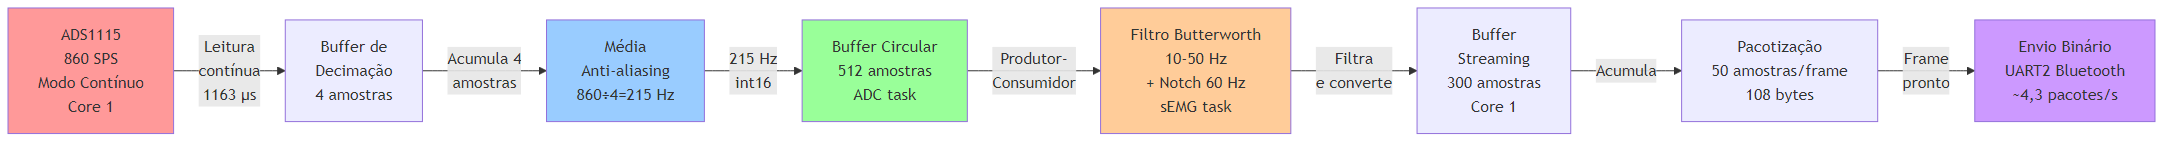
\includegraphics[width=\textwidth]{figuras/Desenvolvimento/NeuroEstimulator/pipeline-aquisicao-decimacao.png}
    \fonte{Autoria própria (2026)}
\end{figure}

% ----------------------------------------------------------------------
\subsubsection{Reorganização das tarefas FreeRTOS}\label{subsubsec:NETarefas}
% ----------------------------------------------------------------------

A operação contínua do estágio de aquisição inviabilizou o modelo original do \textit{firmware}, no qual uma única função de \textit{callback} disparada por temporizador realizava a leitura síncrona do ADC, aplicava o filtro e empacotava o dado para envio via Bluetooth. Esse modelo monolítico bloqueava o núcleo durante o intervalo de leitura I$^2$C do ADS1115 e, sob carga (por exemplo, durante a transmissão de respostas JSON pela mesma UART), provocava perda sistemática de amostras. A solução foi decompor o caminho do dado em uma cadeia produtor-consumidor de três tarefas FreeRTOS distintas, distribuídas entre os dois núcleos do ESP32 e desacopladas por buffers circulares.

No núcleo destinado às operações sensíveis a temporização do estímulo (\textit{Core 0}), permaneceram a tarefa de gestão da sessão de FES (prioridade 20) e a tarefa sensora legada empregada na detecção de gatilho mioelétrico para disparo do estímulo (prioridade 10). No núcleo dedicado à comunicação (\textit{Core 1}) passaram a coexistir três tarefas: a tarefa de tratamento de mensagens Bluetooth (prioridade 20), a tarefa de aquisição contínua do ADC (prioridade 18) e a tarefa de \textit{streaming} de sEMG (prioridade 15). A distribuição de prioridades reflete a hierarquia funcional desejada: o tratamento de comandos do aplicativo precede o consumo de dados do conversor, que por sua vez precede a entrega ao canal de saída. As três tarefas do núcleo de comunicação compartilham os recursos de \textit{hardware} por meio de dois \textit{mutexes}: o \texttt{i2cMutex}, que serializa o acesso ao barramento I$^2$C (compartilhado com o giroscópio MPU6050), e o \texttt{MutexBlu}, que serializa a escrita na UART2 entre a tarefa de \textit{streaming} e o tratador de mensagens, evitando entrelaçamento de \textit{bytes} no canal Bluetooth.

O acoplamento entre as tarefas de aquisição e de \textit{streaming} é feito por um buffer circular de 512 amostras de 16 \textit{bits}, dimensionado para tolerar rajadas de mais de dois segundos sem perda; já o acoplamento entre a etapa de filtragem digital e a pacotização para Bluetooth utiliza um segundo buffer circular de 300 amostras, suficiente para absorver atrasos de transmissão de até aproximadamente 1,4\,segundo. Em ambos os buffers, a estratégia de tratamento de \textit{overflow} é o descarte da amostra mais antiga (\textit{drop-oldest}) com sinalização por \textit{log} limitada a uma ocorrência por segundo, escolha que privilegia a continuidade do fluxo em detrimento da bloqueio do produtor -- um dispositivo de aquisição de sEMG que pausa para esperar o consumidor é, na prática, indistinguível de um dispositivo defeituoso para o operador no aplicativo.

A Figura~\ref{fig:tasksFreertos} apresenta a topologia resultante e destaca as relações produtor-consumidor entre as tarefas. Como melhoria adicional, o procedimento de encerramento das tarefas (\textit{shutdown} cooperativo) foi reescrito para sinalizar uma \textit{flag} volátil de saída e aguardar o término natural da iteração corrente antes de remover a tarefa, em substituição ao \texttt{vTaskDelete} direto que o \textit{firmware} original utilizava. A motivação foi eliminar uma classe específica de defeitos observada em sessões consecutivas de aquisição, na qual a remoção da tarefa em meio a uma transação I$^2$C corrompia o estado interno do barramento e exigia reinicialização física do dispositivo.

\begin{figure}[htb]
    \caption{Topologia das tarefas FreeRTOS no \textit{firmware} adaptado}
    \label{fig:tasksFreertos}
    \centering
    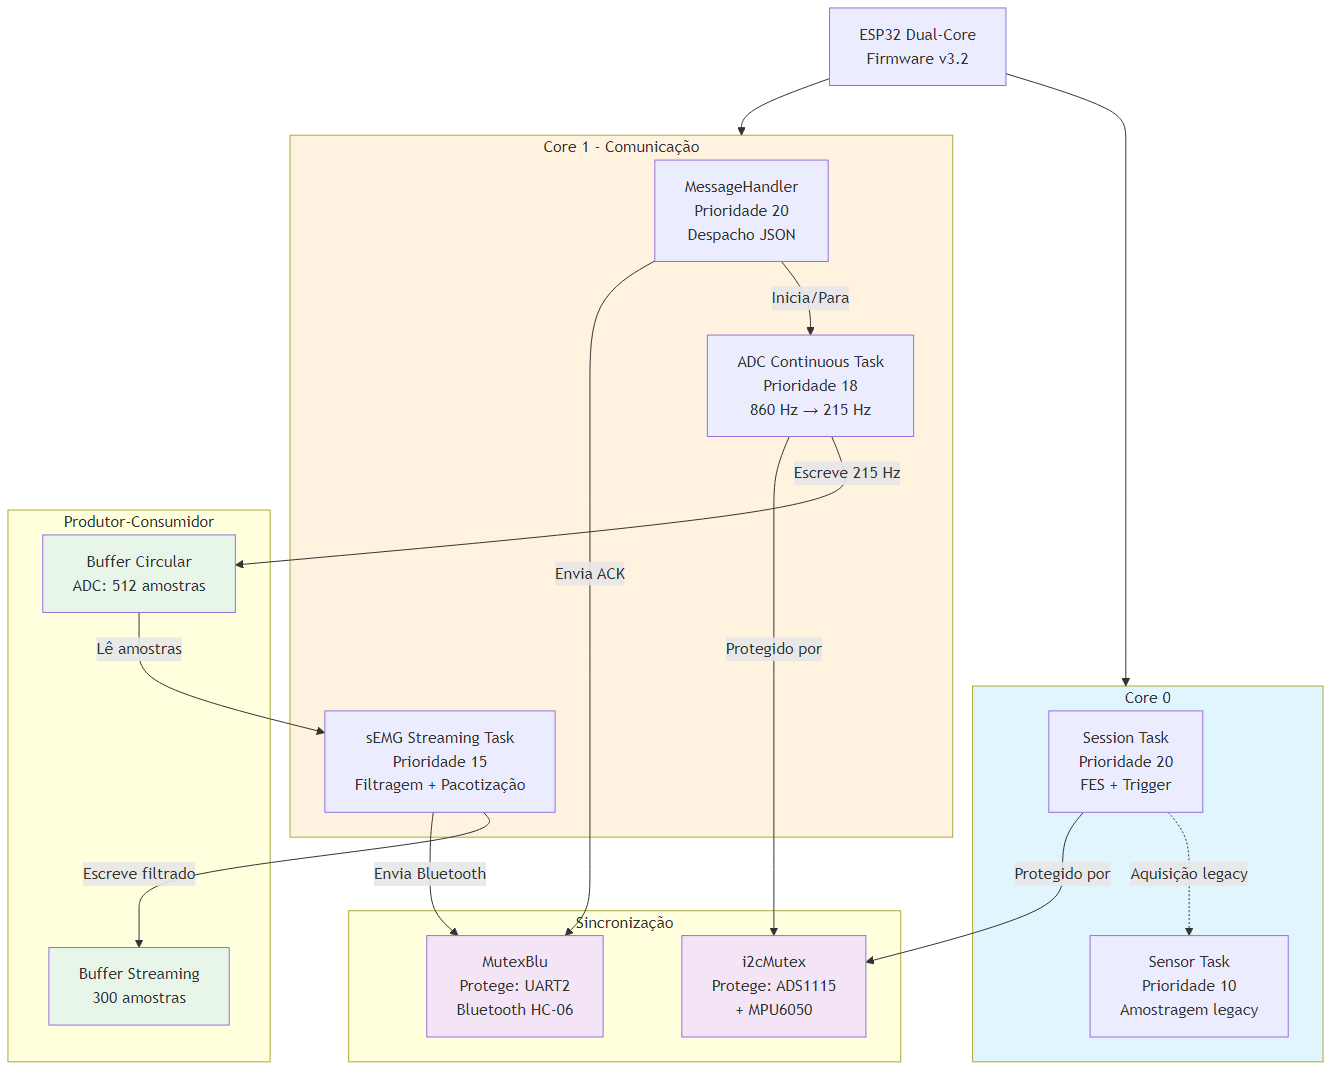
\includegraphics[width=\textwidth]{figuras/Desenvolvimento/NeuroEstimulator/tasks-freertos.png}
    \fonte{Autoria própria (2026)}
\end{figure}

% ----------------------------------------------------------------------
\subsubsection{Protocolo Bluetooth: do comando-resposta ao \textit{streaming}}\label{subsubsec:NEProtocolo}
% ----------------------------------------------------------------------

O protocolo de comunicação do \textit{firmware} original era inteiramente baseado em mensagens JSON encapsuladas em um envelope \verb|{"cd": <code>, "mt": "<method>", "bd": {...}}| trafegando sobre a UART2. Para a aquisição de sEMG, o aplicativo enviava periodicamente uma requisição de leitura e o \textit{firmware} respondia com um pequeno bloco de amostras codificado em JSON. Esse padrão tem dois inconvenientes em uma aplicação de \textit{streaming}: o aplicativo precisa manter um relógio sincronizado com o \textit{firmware} apenas para temporizar suas requisições, e a redundância textual do JSON (chaves de objeto, vírgulas, representação decimal de cada amostra como \textit{string}) consome largura de banda desproporcional à informação efetivamente transportada.

No \textit{firmware} adaptado, o protocolo passou a ser dual: comandos de controle continuam em JSON, mantendo legibilidade e compatibilidade com ferramentas existentes; o fluxo de dados de sEMG, entretanto, é transmitido como uma sequência de pacotes binários enviados de forma autônoma pelo \textit{firmware} entre as transições \texttt{START\_STREAM} e \texttt{STOP\_STREAM}. O aplicativo abre o \textit{streaming} enviando \verb|{"cd":11,"mt":"x"}|, recebe um \textit{acknowledgment} \verb|{"cd":11,"mt":"a"}| e, a partir desse momento, recebe pacotes binários até enviar \verb|{"cd":12,"mt":"x"}| para encerrar. A transição inversa -- voltar a um modelo comando-resposta para o canal de dados -- foi descartada como design alternativo, em razão das desvantagens já discutidas; a configuração de taxa em tempo de execução, presente em uma versão intermediária do \textit{firmware} sob o código de mensagem \texttt{cd:14}, também foi removida, em favor da configuração fixa de 215\,SPS discutida na Subseção~\ref{subsubsec:NEDecimacao}. O Quadro~\ref{quad:campos-pacote-binario} descreve os campos do novo \textit{frame} de dados, e a Figura~\ref{fig:pacoteBinario} ilustra graficamente seu \textit{layout}.

\begin{table}[htb]
    \centering
    \caption{Quadro -- Campos do pacote binário de \textit{streaming} de sEMG}\label{tab:campos-pacote-binario}
    \begin{tabular}{|c|c|l|p{6cm}|}
        \hline
        \textbf{Offset} & \textbf{Tamanho} & \textbf{Campo} & \textbf{Descrição} \\
        \hline
        0 & 1 \textit{byte} & \texttt{magic} & Marcador de início de pacote (valor fixo \texttt{0xAA}). \\
        \hline
        1 & 1 \textit{byte} & \texttt{message\_code} & Código do tipo de mensagem (valor fixo \texttt{0x0D}, dados de \textit{stream}). \\
        \hline
        2 & 4 \textit{bytes} & \texttt{timestamp} & Valor de \texttt{millis()} no ESP32, em \textit{little-endian}. \\
        \hline
        6 & 2 \textit{bytes} & \texttt{sample\_count} & Número de amostras no \textit{payload} (tipicamente 50). \\
        \hline
        8 & 100 \textit{bytes} & \texttt{samples[]} & 50 valores \texttt{int16\_t} em \textit{little-endian} (1\,LSB $\equiv$ 1\,mV). \\
        \hline
        \multicolumn{2}{|c|}{\textbf{Total: 108 \textit{bytes}}} & \multicolumn{2}{l|}{\textit{Frame} fixo enviado a $\approx$\,4,3 pacotes/s.} \\
        \hline
    \end{tabular}
    \fonte{Autoria própria (2026)}
\end{table}

\begin{figure}[htb]
    \caption{\textit{Layout} binário do pacote de \textit{streaming}}
    \label{fig:pacoteBinario}
    \centering
    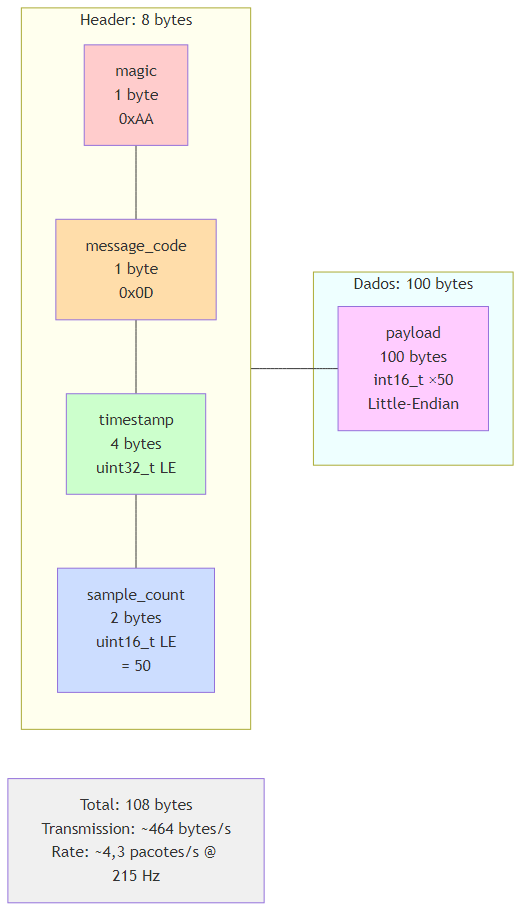
\includegraphics[width=0.95\textwidth]{figuras/Desenvolvimento/NeuroEstimulator/pacote-binario.png}
    \fonte{Autoria própria (2026)}
\end{figure}

A Figura~\ref{fig:protocoloStreaming} resume o diálogo completo entre o IRIS Mobile, o tratador de mensagens, as tarefas internas do \textit{firmware} e o canal Bluetooth durante uma sessão de aquisição.

\begin{figure}[htb]
    \caption{Diagrama de sequência do \textit{streaming} de sEMG entre o IRIS Mobile e o \textit{firmware} adaptado}
    \label{fig:protocoloStreaming}
    \centering
    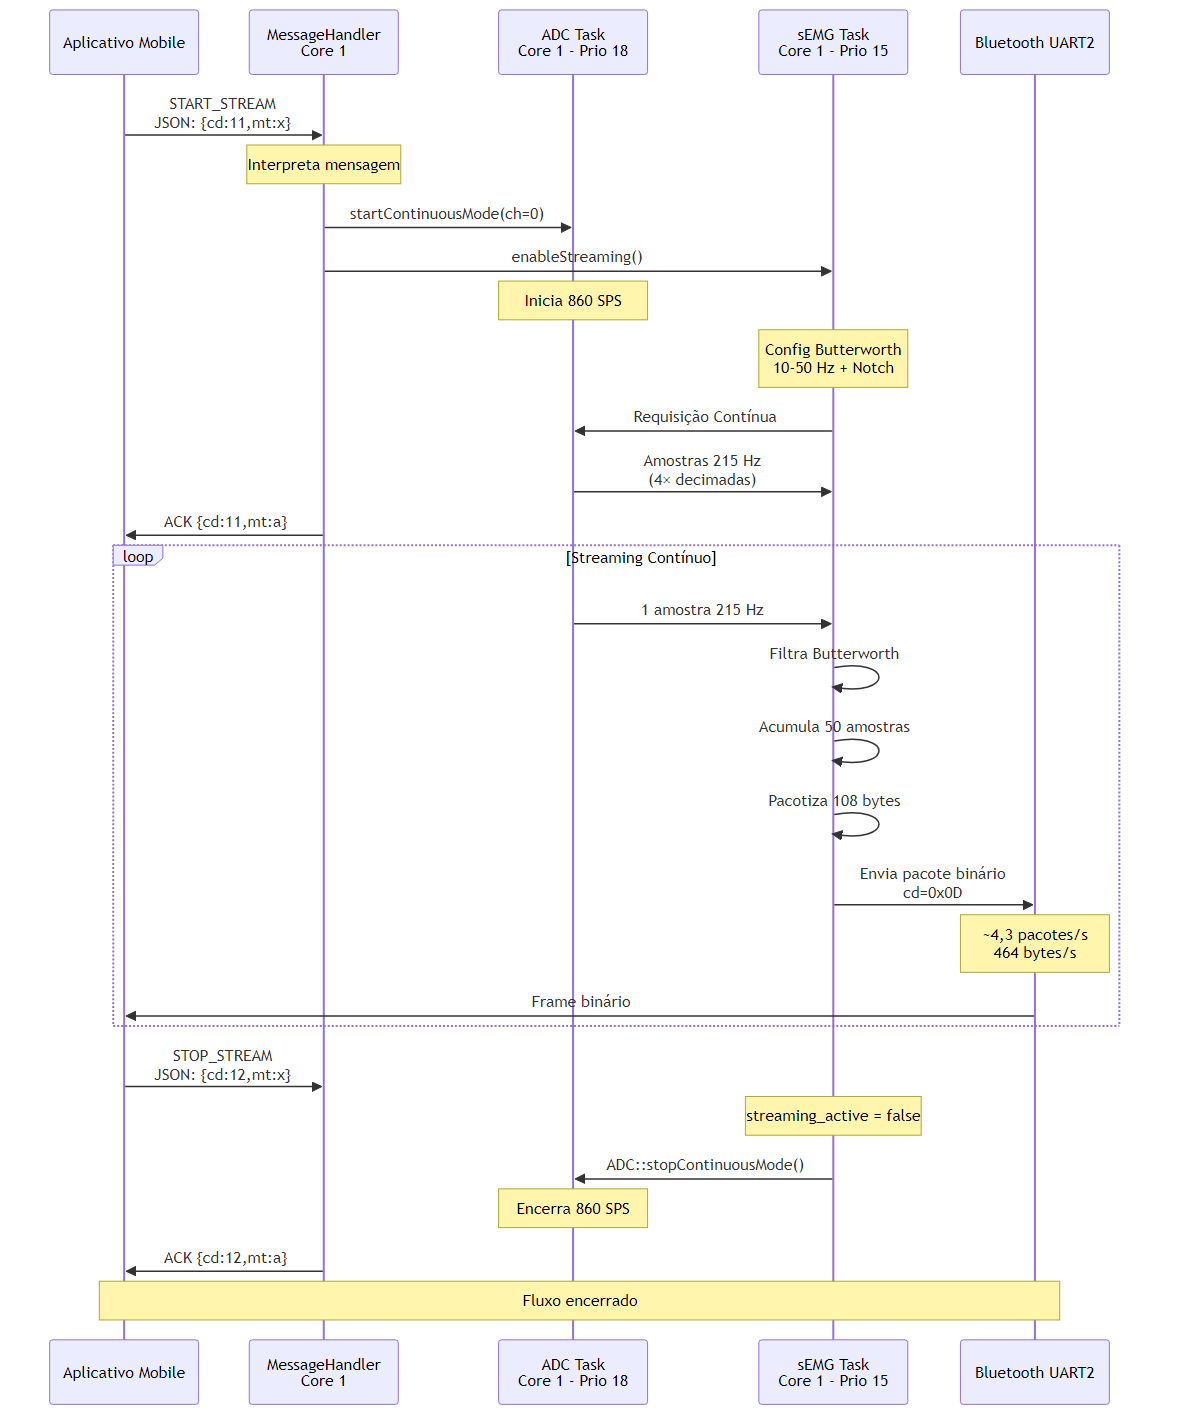
\includegraphics[width=\textwidth]{figuras/Desenvolvimento/NeuroEstimulator/protocolo-streaming.png}
    \fonte{Autoria própria (2026)}
\end{figure}

A escolha de codificar cada amostra em \texttt{int16\_t}, em vez de ponto flutuante, e de \textit{little-endian} como ordem de \textit{bytes} foi guiada por três critérios: a preservação da precisão útil do sinal (a granularidade do ADS1115 a 16~\textit{bits} permite representar tensões em milivolts inteiros sem perda significativa para a aplicação); a economia de banda em relação às alternativas textuais (a transmissão equivalente em JSON consumiria mais do que o triplo da capacidade do canal a 215\,SPS); e a interoperabilidade com a arquitetura nativa do ESP32 e dos dispositivos móveis modernos, que são predominantemente \textit{little-endian} -- o que evita conversões de ordem de \textit{byte} no consumidor. A compatibilidade retroativa com o protocolo JSON anterior para o canal de dados foi descartada de forma deliberada: aplicações que ainda dependam do formato textual podem consumir o canal de controle, mas o IRIS Mobile e o NPI consomem exclusivamente o protocolo binário aqui descrito.

% ======================================================================
% Lista de placeholders de imagens sugeridas (referência interna -- não
% renderizada). Cada item indica o caminho esperado e o que a imagem
% deve mostrar:
% ----------------------------------------------------------------------
% [1] figuras/Desenvolvimento/NeuroEstimulator/neuroestimulador-foto.jpg
%     Foto frontal do dispositivo NeuroEstimulator (caixa MDF, botão de
%     emergência, LEDs de status, conectores). Sugestão: reaproveitar a
%     Figura 7 do Technical Report -- Integration Workshop 3 (2023) ou
%     produzir uma fotografia atualizada. Referenciada (em comentário) em
%     \subsec{NEOriginal}.
%
% [2] figuras/Desenvolvimento/NeuroEstimulator/pipeline-aquisicao-decimacao.png
%     Renderização PNG do diagrama Mermaid pipeline-aquisicao-decimacao.mmd
%     (já existente). Mostra ADS1115 -> média 4x -> buffer circular ->
%     filtros -> buffer streaming -> pacote binário -> Bluetooth.
%
% [3] figuras/Desenvolvimento/NeuroEstimulator/tasks-freertos.png
%     Renderização PNG do diagrama Mermaid tasks-freertos.mmd
%     (já existente). Mostra topologia FreeRTOS pos-refatoracao,
%     com Core 0 / Core 1, prioridades e mutexes.
%
% [4] figuras/Desenvolvimento/NeuroEstimulator/protocolo-streaming.png
%     Renderização PNG do diagrama Mermaid protocolo-streaming.mmd
%     (já existente). Mostra sequencia START_STREAM -> ACK -> pacotes
%     binarios autonomos -> STOP_STREAM -> ACK.
%
% [5] figuras/Desenvolvimento/NeuroEstimulator/pacote-binario.png
%     Renderização PNG do diagrama Mermaid pacote-binario.mmd
%     (já existente). Mostra layout do frame de 108 bytes com header
%     (magic, code, timestamp, sample_count) e payload (50 x int16_t).
% ======================================================================

% =====================================================================

\section{Adaptação do NeuroEstimulator}\label{sec:adaptacaoNeuroEstimulator}

O NeuroEstimulator descrito na Seção~\ref{sec:coletaDeDados} foi adotado, no presente trabalho, como dispositivo-exemplo para validar a integração de equipamentos de aquisição de biossinais ao PRISM. A descrição original do projeto -- mecânica, eletrônica, escolha de componentes e arquitetura geral do firmware -- não é repetida aqui; esta seção concentra-se exclusivamente nas \textbf{modificações} introduzidas para tornar o dispositivo compatível com o fluxo de etiquetagem em tempo real previsto pelo IRIS Mobile e, consequentemente, com o modelo de coleta padronizado proposto pelo PRISM. As alterações foram restritas ao firmware e ao protocolo de comunicação Bluetooth: nenhuma modificação foi feita na placa de circuito impresso, no \textit{front-end} analógico, no transformador 1:10 ou nos elementos mecânicos do equipamento.

% ----------------------------------------------------------------------
\subsection{O dispositivo original}\label{subsec:NEOriginal}
% ----------------------------------------------------------------------

Para fins de contextualização, recapitulam-se aqui apenas os elementos do dispositivo original relevantes para a adaptação. O NeuroEstimulator é um sistema funcional de eletroestimulação descrito em detalhes na Seção~\ref{sec:coletaDeDados}, organizado em torno de um microcontrolador ESP32 (arquitetura Xtensa LX6 \textit{dual-core}), \textit{front-end} analógico AD8232 dedicado à condicionamento do sinal de eletromiografia de superfície (sEMG), conversor analógico-digital ADS1115 (16 bits de resolução, taxa máxima de 860 amostras por segundo na configuração utilizada) e módulo Bluetooth Classic HC-06 acoplado à UART2. O \textit{firmware} originalmente embarcado opera sobre o sistema operacional de tempo real FreeRTOS, distribuindo entre os dois núcleos do ESP32 as tarefas de gestão de sessão, geração de pulsos de estimulação elétrica funcional (FES, do inglês \textit{Functional Electrical Stimulation}) e leitura periódica do sEMG.

% Imagem sugerida: foto do dispositivo montado (caixa MDF + PCB + suportes).
% Este placeholder permite reutilizar a Figura~7 do relatório técnico do
% Workshop de Integração 3 (NeuroEstimulator, 2023) ou capturar uma nova
% fotografia atualizada do equipamento.
%
% \begin{figure}[htb]
%     \caption{Visão externa do NeuroEstimulator utilizado como dispositivo-exemplo}
%     \label{fig:neuroEstimuladorExterno}
%     \centering
%     \includegraphics[width=0.7\textwidth]{figuras/Desenvolvimento/NeuroEstimulator/neuroestimulador-foto.jpg}
%     \fonte{}
% \end{figure}

% ----------------------------------------------------------------------
\subsection{Diferencial pretendido para o trabalho}\label{subsec:NERequisitos}
% ----------------------------------------------------------------------

A adoção do NeuroEstimulator como dispositivo-exemplo do PRISM exigiu uma reformulação parcial do \textit{firmware} para satisfazer requisitos que não eram contemplados pelo projeto original. Esses requisitos derivam diretamente do modelo de coleta proposto, em que o sinal de sEMG precisa ser exibido e etiquetado em tempo real pelo IRIS Mobile durante a sessão. As principais diretrizes que motivaram a refatoração foram:

\begin{enumerate}
    \item \textbf{Maximizar a taxa efetiva de amostragem entregue ao aplicativo}, aproximando-a do limite teórico do conversor empregado e estabilizando-a em um valor previsível. Na implementação anterior do \textit{firmware}, o pareamento entre o temporizador de amostragem e a leitura síncrona do ADS1115 causava bloqueios da ordem de milissegundos, fazendo com que apenas uma fração das amostras nominalmente programadas chegasse efetivamente ao aplicativo;
    \item \textbf{Substituir o protocolo do tipo comando-resposta} por uma transmissão contínua orientada a fluxo (\textit{streaming}), de modo que cada amostra coletada seja entregue ao consumidor sem necessidade de requisição explícita;
    \item \textbf{Tornar o contrato de comunicação compatível com a etiquetagem em tempo real} prevista pelo IRIS Mobile, agregando carimbo de tempo (\textit{timestamp}) consistente em cada bloco de amostras e reduzindo a sobrecarga de transporte para que o canal serial Bluetooth não se tornasse o gargalo do sistema;
    \item \textbf{Manter a compatibilidade com o \textit{hardware} existente}, sem qualquer alteração na placa, no \textit{front-end} analógico, no estágio de potência da estimulação ou no módulo Bluetooth Classic já instalado.
\end{enumerate}

Os três primeiros requisitos pertencem ao domínio do \textit{software} embarcado e do protocolo. O quarto é uma restrição de projeto que limita o universo de soluções possíveis -- em particular, ele inviabiliza a substituição do ADS1115 por um conversor de taxa mais alta e impede a troca do HC-06 por um módulo Bluetooth Low Energy ou Wi-Fi de maior largura de banda.

% ----------------------------------------------------------------------
\subsection{Modificações no firmware}\label{subsec:NEFirmware}
% ----------------------------------------------------------------------

As modificações no \textit{firmware} foram organizadas em três frentes complementares, descritas nas próximas subseções: a reconfiguração do estágio de aquisição para operar em modo contínuo com decimação interna; a reorganização das tarefas FreeRTOS em um pipeline produtor-consumidor; e a substituição do protocolo Bluetooth comando-resposta por um \textit{streaming} binário com cabeçalho fixo.

% ----------------------------------------------------------------------
\subsubsection{Aquisição contínua a 860 SPS e decimação para 215 SPS}\label{subsubsec:NEDecimacao}
% ----------------------------------------------------------------------

A taxa efetiva de saída do estágio de aquisição foi fixada em 215 amostras por segundo (\textit{samples per second}, SPS), obtida a partir de uma operação contínua do ADS1115 a 860 SPS seguida de uma decimação 4:1 por média móvel. A escolha de 860 SPS como ponto de operação não é arbitrária: trata-se da maior taxa nominal disponível no ADS1115 quando configurado em modo de conversão contínua com a faixa de tensão de entrada utilizada pelo NeuroEstimulator. Operar abaixo desse teto deixaria capacidade ociosa do conversor; tentar ultrapassá-lo simplesmente não é suportado pelo \textit{hardware}.

A decimação 4:1 por média foi adotada por três razões. A primeira é o seu efeito como filtro \textit{anti-aliasing} simples: o cálculo da média de quatro amostras consecutivas atenua componentes de alta frequência antes que o sinal seja entregue à etapa de filtragem digital, reduzindo a probabilidade de \textit{aliasing} causado por ruído eletromagnético do ambiente clínico. A segunda razão é a obtenção de uma relação 1:1 entre amostras lidas e amostras entregues que respeita os limites de banda exigidos pelo canal Bluetooth Classic: a 215 SPS, com codificação binária compacta, a vazão de saída fica em torno de 464 \textit{bytes} por segundo, o que corresponde a aproximadamente 4\% da capacidade nominal da UART2 configurada a 115\,200 \textit{baud}, deixando uma margem confortável para retransmissões e tráfego de controle. A terceira razão é simplificar a configuração do filtro digital: ao fixar a taxa de entrega em 215 SPS, os coeficientes do filtro Butterworth de segunda ordem (passa-faixa de 10\,Hz a 50\,Hz) e do \textit{notch} de 60\,Hz para rejeição de interferência da rede elétrica podem ser pré-calculados em tempo de compilação, eliminando uma fonte recorrente de erros que o \textit{firmware} original apresentava ao reconfigurar dinamicamente a taxa.

É necessário, contudo, discutir honestamente a contrapartida dessa escolha. A literatura de eletromiografia indica que a banda útil do sEMG de superfície estende-se aproximadamente entre 10\,Hz e 500\,Hz. Pelo critério de Nyquist, uma taxa de amostragem efetiva de 215 SPS limita a banda passível de reconstrução fiel a aproximadamente 107,5\,Hz, valor inferior ao extremo superior da banda fisiológica do sEMG. A decisão arquitetural foi privilegiar a faixa entre 10\,Hz e 50\,Hz, onde se concentra a maior parte da energia do sinal mioelétrico utilizado para detecção de ativação muscular, em detrimento da captura de componentes de mais alta frequência. Esta limitação é uma decorrência direta da restrição de não modificar o \textit{hardware} (Subseção~\ref{subsec:NERequisitos}, requisito 4); ela é retomada no capítulo de discussão dos resultados à luz dos sinais efetivamente capturados, e deve ser entendida como uma limitação reconhecida do dispositivo-exemplo, não uma propriedade do PRISM.

A Figura~\ref{fig:pipelineAquisicaoDecimacao} resume o caminho do dado desde o conversor analógico-digital até a saída pelo módulo Bluetooth.

\begin{figure}[htb]
    \caption{Pipeline de aquisição, decimação e filtragem do sEMG no \textit{firmware} adaptado}
    \label{fig:pipelineAquisicaoDecimacao}
    \centering
    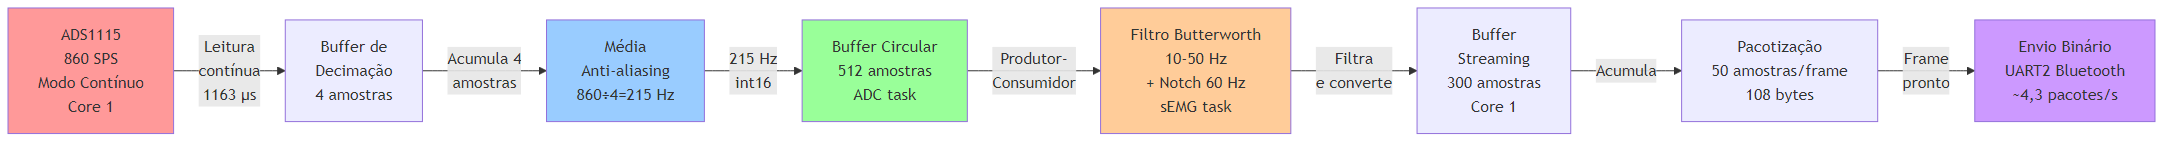
\includegraphics[width=\textwidth]{figuras/Desenvolvimento/NeuroEstimulator/pipeline-aquisicao-decimacao.png}
    \fonte{Autoria própria (2026)}
\end{figure}

% ----------------------------------------------------------------------
\subsubsection{Reorganização das tarefas FreeRTOS}\label{subsubsec:NETarefas}
% ----------------------------------------------------------------------

A operação contínua do estágio de aquisição inviabilizou o modelo original do \textit{firmware}, no qual uma única função de \textit{callback} disparada por temporizador realizava a leitura síncrona do ADC, aplicava o filtro e empacotava o dado para envio via Bluetooth. Esse modelo monolítico bloqueava o núcleo durante o intervalo de leitura I$^2$C do ADS1115 e, sob carga (por exemplo, durante a transmissão de respostas JSON pela mesma UART), provocava perda sistemática de amostras. A solução foi decompor o caminho do dado em uma cadeia produtor-consumidor de três tarefas FreeRTOS distintas, distribuídas entre os dois núcleos do ESP32 e desacopladas por buffers circulares.

No núcleo destinado às operações sensíveis a temporização do estímulo (\textit{Core 0}), permaneceram a tarefa de gestão da sessão de FES (prioridade 20) e a tarefa sensora legada empregada na detecção de gatilho mioelétrico para disparo do estímulo (prioridade 10). No núcleo dedicado à comunicação (\textit{Core 1}) passaram a coexistir três tarefas: a tarefa de tratamento de mensagens Bluetooth (prioridade 20), a tarefa de aquisição contínua do ADC (prioridade 18) e a tarefa de \textit{streaming} de sEMG (prioridade 15). A distribuição de prioridades reflete a hierarquia funcional desejada: o tratamento de comandos do aplicativo precede o consumo de dados do conversor, que por sua vez precede a entrega ao canal de saída. As três tarefas do núcleo de comunicação compartilham os recursos de \textit{hardware} por meio de dois \textit{mutexes}: o \texttt{i2cMutex}, que serializa o acesso ao barramento I$^2$C (compartilhado com o giroscópio MPU6050), e o \texttt{MutexBlu}, que serializa a escrita na UART2 entre a tarefa de \textit{streaming} e o tratador de mensagens, evitando entrelaçamento de \textit{bytes} no canal Bluetooth.

O acoplamento entre as tarefas de aquisição e de \textit{streaming} é feito por um buffer circular de 512 amostras de 16 \textit{bits}, dimensionado para tolerar rajadas de mais de dois segundos sem perda; já o acoplamento entre a etapa de filtragem digital e a pacotização para Bluetooth utiliza um segundo buffer circular de 300 amostras, suficiente para absorver atrasos de transmissão de até aproximadamente 1,4\,segundo. Em ambos os buffers, a estratégia de tratamento de \textit{overflow} é o descarte da amostra mais antiga (\textit{drop-oldest}) com sinalização por \textit{log} limitada a uma ocorrência por segundo, escolha que privilegia a continuidade do fluxo em detrimento da bloqueio do produtor -- um dispositivo de aquisição de sEMG que pausa para esperar o consumidor é, na prática, indistinguível de um dispositivo defeituoso para o operador no aplicativo.

A Figura~\ref{fig:tasksFreertos} apresenta a topologia resultante e destaca as relações produtor-consumidor entre as tarefas. Como melhoria adicional, o procedimento de encerramento das tarefas (\textit{shutdown} cooperativo) foi reescrito para sinalizar uma \textit{flag} volátil de saída e aguardar o término natural da iteração corrente antes de remover a tarefa, em substituição ao \texttt{vTaskDelete} direto que o \textit{firmware} original utilizava. A motivação foi eliminar uma classe específica de defeitos observada em sessões consecutivas de aquisição, na qual a remoção da tarefa em meio a uma transação I$^2$C corrompia o estado interno do barramento e exigia reinicialização física do dispositivo.

\begin{figure}[htb]
    \caption{Topologia das tarefas FreeRTOS no \textit{firmware} adaptado}
    \label{fig:tasksFreertos}
    \centering
    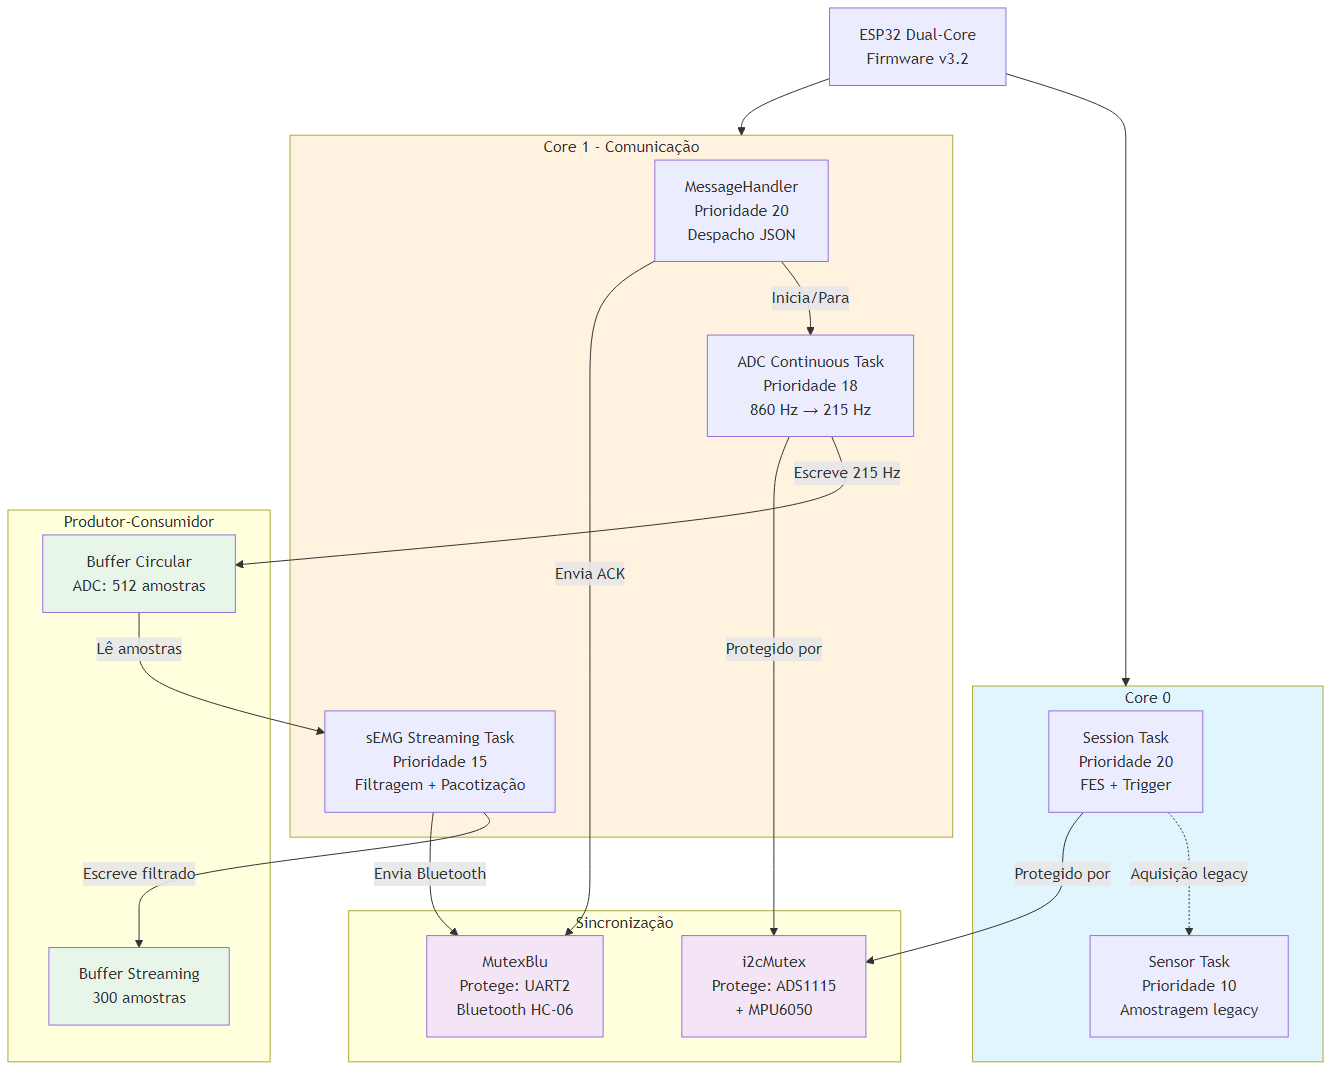
\includegraphics[width=\textwidth]{figuras/Desenvolvimento/NeuroEstimulator/tasks-freertos.png}
    \fonte{Autoria própria (2026)}
\end{figure}

% ----------------------------------------------------------------------
\subsubsection{Protocolo Bluetooth: do comando-resposta ao \textit{streaming}}\label{subsubsec:NEProtocolo}
% ----------------------------------------------------------------------

O protocolo de comunicação do \textit{firmware} original era inteiramente baseado em mensagens JSON encapsuladas em um envelope \verb|{"cd": <code>, "mt": "<method>", "bd": {...}}| trafegando sobre a UART2. Para a aquisição de sEMG, o aplicativo enviava periodicamente uma requisição de leitura e o \textit{firmware} respondia com um pequeno bloco de amostras codificado em JSON. Esse padrão tem dois inconvenientes em uma aplicação de \textit{streaming}: o aplicativo precisa manter um relógio sincronizado com o \textit{firmware} apenas para temporizar suas requisições, e a redundância textual do JSON (chaves de objeto, vírgulas, representação decimal de cada amostra como \textit{string}) consome largura de banda desproporcional à informação efetivamente transportada.

No \textit{firmware} adaptado, o protocolo passou a ser dual: comandos de controle continuam em JSON, mantendo legibilidade e compatibilidade com ferramentas existentes; o fluxo de dados de sEMG, entretanto, é transmitido como uma sequência de pacotes binários enviados de forma autônoma pelo \textit{firmware} entre as transições \texttt{START\_STREAM} e \texttt{STOP\_STREAM}. O aplicativo abre o \textit{streaming} enviando \verb|{"cd":11,"mt":"x"}|, recebe um \textit{acknowledgment} \verb|{"cd":11,"mt":"a"}| e, a partir desse momento, recebe pacotes binários até enviar \verb|{"cd":12,"mt":"x"}| para encerrar. A transição inversa -- voltar a um modelo comando-resposta para o canal de dados -- foi descartada como design alternativo, em razão das desvantagens já discutidas; a configuração de taxa em tempo de execução, presente em uma versão intermediária do \textit{firmware} sob o código de mensagem \texttt{cd:14}, também foi removida, em favor da configuração fixa de 215\,SPS discutida na Subseção~\ref{subsubsec:NEDecimacao}. O Quadro~\ref{quad:campos-pacote-binario} descreve os campos do novo \textit{frame} de dados, e a Figura~\ref{fig:pacoteBinario} ilustra graficamente seu \textit{layout}.

\begin{table}[htb]
    \centering
    \caption{Quadro -- Campos do pacote binário de \textit{streaming} de sEMG}\label{tab:campos-pacote-binario}
    \begin{tabular}{|c|c|l|p{6cm}|}
        \hline
        \textbf{Offset} & \textbf{Tamanho} & \textbf{Campo} & \textbf{Descrição} \\
        \hline
        0 & 1 \textit{byte} & \texttt{magic} & Marcador de início de pacote (valor fixo \texttt{0xAA}). \\
        \hline
        1 & 1 \textit{byte} & \texttt{message\_code} & Código do tipo de mensagem (valor fixo \texttt{0x0D}, dados de \textit{stream}). \\
        \hline
        2 & 4 \textit{bytes} & \texttt{timestamp} & Valor de \texttt{millis()} no ESP32, em \textit{little-endian}. \\
        \hline
        6 & 2 \textit{bytes} & \texttt{sample\_count} & Número de amostras no \textit{payload} (tipicamente 50). \\
        \hline
        8 & 100 \textit{bytes} & \texttt{samples[]} & 50 valores \texttt{int16\_t} em \textit{little-endian} (1\,LSB $\equiv$ 1\,mV). \\
        \hline
        \multicolumn{2}{|c|}{\textbf{Total: 108 \textit{bytes}}} & \multicolumn{2}{l|}{\textit{Frame} fixo enviado a $\approx$\,4,3 pacotes/s.} \\
        \hline
    \end{tabular}
    \fonte{Autoria própria (2026)}
\end{table}

\begin{figure}[htb]
    \caption{\textit{Layout} binário do pacote de \textit{streaming}}
    \label{fig:pacoteBinario}
    \centering
    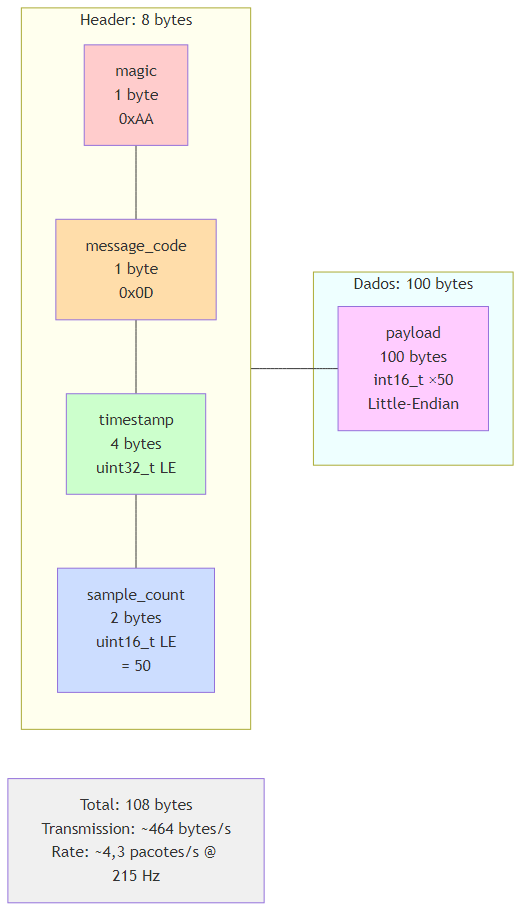
\includegraphics[width=0.95\textwidth]{figuras/Desenvolvimento/NeuroEstimulator/pacote-binario.png}
    \fonte{Autoria própria (2026)}
\end{figure}

A Figura~\ref{fig:protocoloStreaming} resume o diálogo completo entre o IRIS Mobile, o tratador de mensagens, as tarefas internas do \textit{firmware} e o canal Bluetooth durante uma sessão de aquisição.

\begin{figure}[htb]
    \caption{Diagrama de sequência do \textit{streaming} de sEMG entre o IRIS Mobile e o \textit{firmware} adaptado}
    \label{fig:protocoloStreaming}
    \centering
    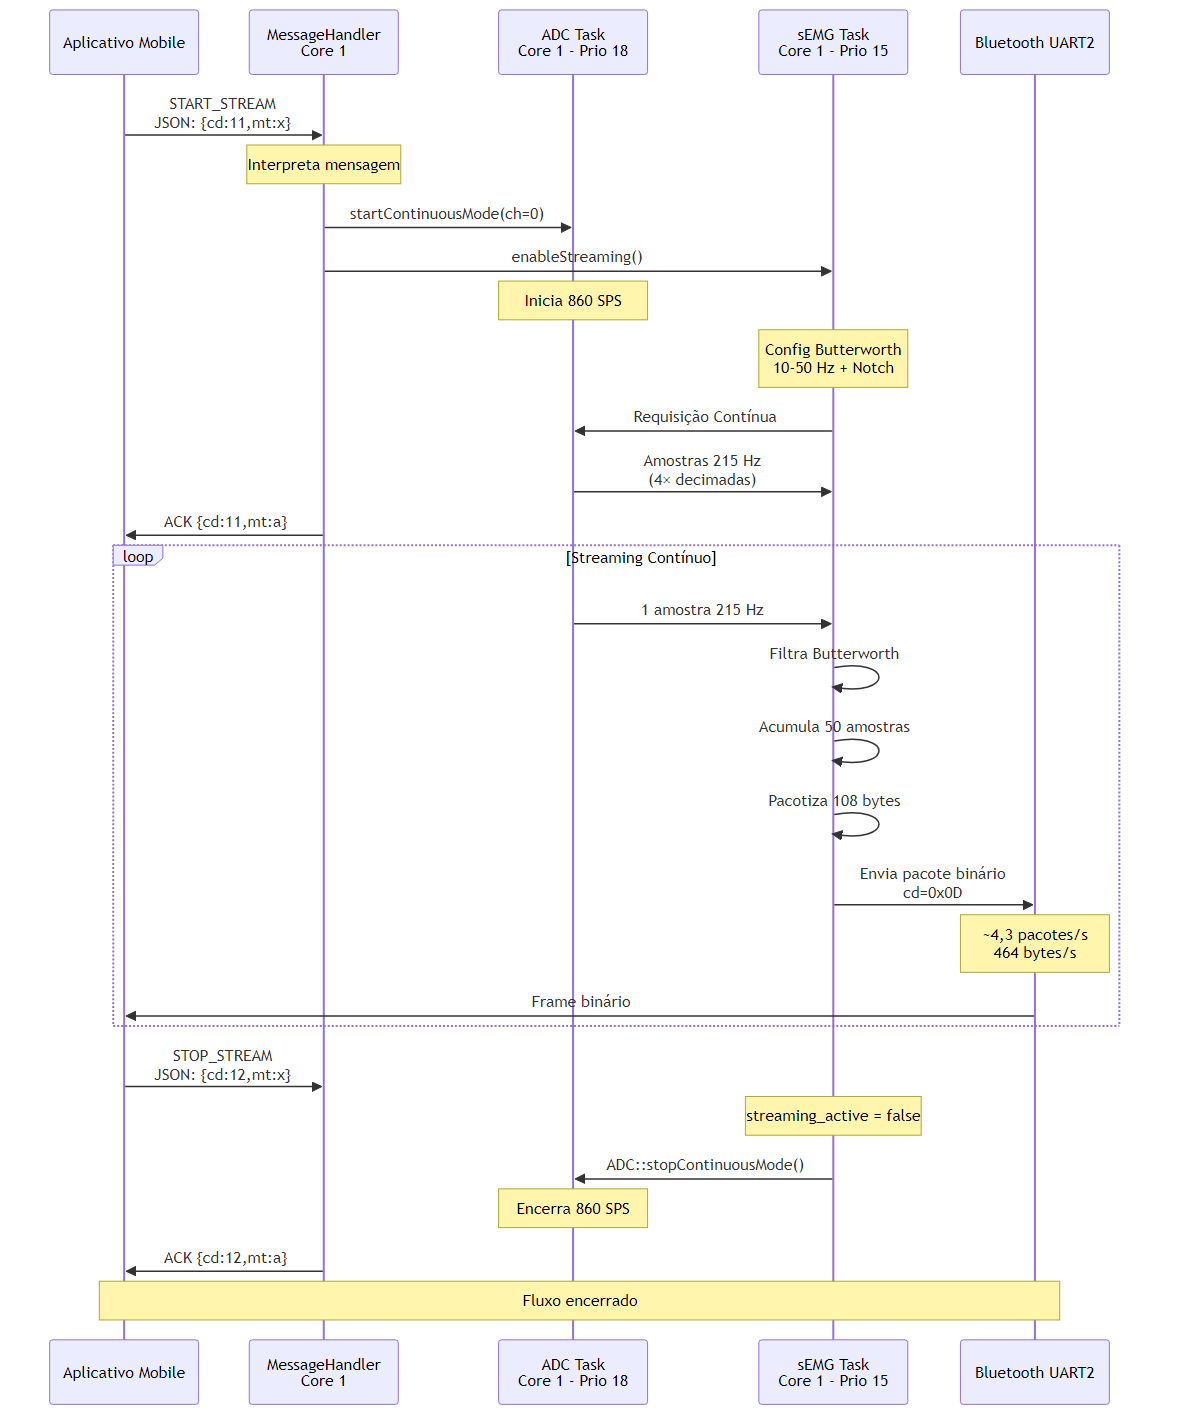
\includegraphics[width=\textwidth]{figuras/Desenvolvimento/NeuroEstimulator/protocolo-streaming.png}
    \fonte{Autoria própria (2026)}
\end{figure}

A escolha de codificar cada amostra em \texttt{int16\_t}, em vez de ponto flutuante, e de \textit{little-endian} como ordem de \textit{bytes} foi guiada por três critérios: a preservação da precisão útil do sinal (a granularidade do ADS1115 a 16~\textit{bits} permite representar tensões em milivolts inteiros sem perda significativa para a aplicação); a economia de banda em relação às alternativas textuais (a transmissão equivalente em JSON consumiria mais do que o triplo da capacidade do canal a 215\,SPS); e a interoperabilidade com a arquitetura nativa do ESP32 e dos dispositivos móveis modernos, que são predominantemente \textit{little-endian} -- o que evita conversões de ordem de \textit{byte} no consumidor. A compatibilidade retroativa com o protocolo JSON anterior para o canal de dados foi descartada de forma deliberada: aplicações que ainda dependam do formato textual podem consumir o canal de controle, mas o IRIS Mobile e o NPI consomem exclusivamente o protocolo binário aqui descrito.

% ======================================================================
% Lista de placeholders de imagens sugeridas (referência interna -- não
% renderizada). Cada item indica o caminho esperado e o que a imagem
% deve mostrar:
% ----------------------------------------------------------------------
% [1] figuras/Desenvolvimento/NeuroEstimulator/neuroestimulador-foto.jpg
%     Foto frontal do dispositivo NeuroEstimulator (caixa MDF, botão de
%     emergência, LEDs de status, conectores). Sugestão: reaproveitar a
%     Figura 7 do Technical Report -- Integration Workshop 3 (2023) ou
%     produzir uma fotografia atualizada. Referenciada (em comentário) em
%     \subsec{NEOriginal}.
%
% [2] figuras/Desenvolvimento/NeuroEstimulator/pipeline-aquisicao-decimacao.png
%     Renderização PNG do diagrama Mermaid pipeline-aquisicao-decimacao.mmd
%     (já existente). Mostra ADS1115 -> média 4x -> buffer circular ->
%     filtros -> buffer streaming -> pacote binário -> Bluetooth.
%
% [3] figuras/Desenvolvimento/NeuroEstimulator/tasks-freertos.png
%     Renderização PNG do diagrama Mermaid tasks-freertos.mmd
%     (já existente). Mostra topologia FreeRTOS pos-refatoracao,
%     com Core 0 / Core 1, prioridades e mutexes.
%
% [4] figuras/Desenvolvimento/NeuroEstimulator/protocolo-streaming.png
%     Renderização PNG do diagrama Mermaid protocolo-streaming.mmd
%     (já existente). Mostra sequencia START_STREAM -> ACK -> pacotes
%     binarios autonomos -> STOP_STREAM -> ACK.
%
% [5] figuras/Desenvolvimento/NeuroEstimulator/pacote-binario.png
%     Renderização PNG do diagrama Mermaid pacote-binario.mmd
%     (já existente). Mostra layout do frame de 108 bytes com header
%     (magic, code, timestamp, sample_count) e payload (50 x int16_t).
% ======================================================================
